%%%%%%%%%%%%%%%%%%%%%%%%%%%%%%%%%%%%%%%%%%%%%%%%%%%%%%%%%%%%%%%%%%%%%%%%%%%%%%%%
%
% Template license:
% CC BY-NC-SA 3.0 (http://creativecommons.org/licenses/by-nc-sa/3.0/)
%
%%%%%%%%%%%%%%%%%%%%%%%%%%%%%%%%%%%%%%%%%%%%%%%%%%%%%%%%%%%%%%%%%%%%%%%%%%%%%%%%

%----------------------------------------------------------------------------------------
%	PACKAGES AND OTHER DOCUMENT CONFIGURATIONS
%----------------------------------------------------------------------------------------

\documentclass[
11pt, % The default document font size, options: 10pt, 11pt, 12pt
%oneside, % Two side (alternating margins) for binding by default, uncomment to switch to one side
%chapterinoneline,% Have the chapter title next to the number in one single line
spanish,
singlespacing, % Single line spacing, alternatives: onehalfspacing or doublespacing
%draft, % Uncomment to enable draft mode (no pictures, no links, overfull hboxes indicated)
%nolistspacing, % If the document is onehalfspacing or doublespacing, uncomment this to set spacing in lists to single
%liststotoc, % Uncomment to add the list of figures/tables/etc to the table of contents
%toctotoc, % Uncomment to add the main table of contents to the table of contents
parskip, % Uncomment to add space between paragraphs
%codirector, % Uncomment to add a codirector to the title page
headsepline, % Uncomment to get a line under the header
]{MastersDoctoralThesis} % The class file specifying the document structure



%----------------------------------------------------------------------------------------
%	INFORMACIÓN DE LA MEMORIA
%----------------------------------------------------------------------------------------

\thesistitle{Modelo de generación automática de emails para clientes} % El títulos de la memoria, se usa en la carátula y se puede usar el cualquier lugar del documento con el comando \ttitle

% Nombre del posgrado, se usa en la carátula y se puede usar el cualquier lugar del documento con el comando \degreename
%\posgrado{Carrera de Especialización en Internet de las Cosas} 
\posgrado{Carrera de Especialización en Intelegencia Artificial}
%\posgrado{Maestría en Sistemas Embebidos} 
%\posgrado{Maestría en Internet de las cosas}

\author{Bach. Josselyn Sofía Ordóñez Olazábal} % Tu nombre, se usa en la carátula y se puede usar el cualquier lugar del documento con el comando \authorname

\director{Esp. Dis. Ana Guzmán (FIUBA)} % El nombre del director, se usa en la carátula y se puede usar el cualquier lugar del documento con el comando \dirname
\codirector{Nombre del codirector (pertenencia)} % El nombre del codirector si lo hubiera, se usa en la carátula y se puede usar el cualquier lugar del documento con el comando \codirname.  Para activar este campo se debe descomentar la opción "codirector" en el comando \documentclass, línea 23.

\juradoUNO{Nombre del jurado 1 (pertenencia)} % Nombre y pertenencia del un jurado se usa en la carátula y se puede usar el cualquier lugar del documento con el comando \jur1name
\juradoDOS{Nombre del jurado 2 (pertenencia)} % Nombre y pertenencia del un jurado se usa en la carátula y se puede usar el cualquier lugar del documento con el comando \jur2name
\juradoTRES{Nombre del jurado 3 (pertenencia)} % Nombre y pertenencia del un jurado se usa en la carátula y se puede usar el cualquier lugar del documento con el comando \jur3name

\ciudad{Ciudad Autónoma de Buenos Aires}

\fechaINICIO{diciembre de 2023}
\fechaFINAL{julio de 2024}


\keywords{Sistemas embebidos, FIUBA} % Keywords for your thesis, print it elsewhere with \keywordnames


\begin{document}


\frontmatter % Use roman page numbering style (i, ii, iii, iv...) for the pre-content pages

\pagestyle{plain} % Default to the plain heading style until the thesis style is called for the body content


%----------------------------------------------------------------------------------------
%	RESUMEN - ABSTRACT 
%----------------------------------------------------------------------------------------

\begin{abstract}
\addchaptertocentry{\abstractname} % Add the abstract to the table of contents
%
%The Thesis Abstract is written here (and usually kept to just this page). The page is kept centered vertically so can expand into the blank space above the title too\ldots
\centering

El objetivo del trabajo propuesto es utilizar inteligencia artificial generativa para producir bocetos de email en pocos segundos a partir de los briefs generados por usuarios. Esta solución aprovecha el reciente crecimiento de los grandes modelos de lenguaje para agilizar el proceso de creación de emails del Banco de Crédito del Perú de tal forma que no sean un cuello de botella para las campañas comerciales y comunicación relacional hacia los clientes.

Para el desarrollo de este trabajo se aplicaron los conocimientos de procesamiento de lenguaje natural, aprendizaje de máquina y visión adquiridos dentro de la Especialización en Inteligencia Artificial de la FIUBA. Para crear la interfaz gráfica se aplicaron también conocimientos de desarrollo web de la Especialización en Internet de las Cosas.

\end{abstract}

%----------------------------------------------------------------------------------------
%	CONTENIDO DE LA MEMORIA  - AGRADECIMIENTOS
%----------------------------------------------------------------------------------------

\begin{acknowledgements}
%\addchaptertocentry{\acknowledgementname} % Descomentando esta línea se puede agregar los agradecimientos al índice
\vspace{1.5cm}

Esta sección es para agradecimientos personales y es totalmente \textbf{OPCIONAL}.  

\end{acknowledgements}

%----------------------------------------------------------------------------------------
%	LISTA DE CONTENIDOS/FIGURAS/TABLAS
%----------------------------------------------------------------------------------------

\tableofcontents % Prints the main table of contents

\listoffigures % Prints the list of figures

\listoftables % Prints the list of tables


%----------------------------------------------------------------------------------------
%	CONTENIDO DE LA MEMORIA  - DEDICATORIA
%----------------------------------------------------------------------------------------

\dedicatory{\textbf{Dedicado a mi querida familia, por todo su apoyo.}}  % escribir acá si se desea una dedicatoria

%----------------------------------------------------------------------------------------
%	CONTENIDO DE LA MEMORIA  - CAPÍTULOS
%----------------------------------------------------------------------------------------

\mainmatter % Begin numeric (1,2,3...) page numbering

\pagestyle{thesis} % Return the page headers back to the "thesis" style

% Incluir los capítulos como archivos separados desde la carpeta Chapters

% Chapter 1

\chapter{Introducción general} % Main chapter title

\label{Chapter1} % For referencing the chapter elsewhere, use \ref{Chapter1} 
\label{IntroGeneral}

%----------------------------------------------------------------------------------------

% Define some commands to keep the formatting separated from the content 
\newcommand{\keyword}[1]{\textbf{#1}}
\newcommand{\tabhead}[1]{\textbf{#1}}
\newcommand{\code}[1]{\texttt{#1}}
\newcommand{\file}[1]{\texttt{\bfseries#1}}
\newcommand{\option}[1]{\texttt{\itshape#1}}
\newcommand{\grados}{$^{\circ}$}

%----------------------------------------------------------------------------------------

%\section{Introducción}

En este capítulo se brinda mayor detalle sobre la importancia del trabajo realizado y sus beneficios para el Banco de Crédito del Perú. Adicionalmente, se especifica cuál es el objetivo y el alcance del proyecto. Finalmente, se brinda un breve resumen de los avances tecnológicos más recientes en inteligencia artificial generativa y los retos implicados en su uso.

%----------------------------------------------------------------------------------------
\section{Motivación}

Uno de los principales medios de comunicación dentro del Banco de Crédito del Perú (BCP) es el email. Dentro de la organización existen varios equipos que usan esta herramienta para comunicar campañas a los clientes, promociones, brindar consejos financieros, entre otros objetivos diversos por áreas. Sin embargo, el proceso de creación de los emails maquetados puede tomar entre 5 a 8 días hábiles, y el equipo que recibe estos pedidos tiene capacidad limitada, por lo que se deben priorizar y rechazar algunas solicitudes. Adicionalmente, estos emails son estáticos y difíciles de personalizar por la carga que conlleva realizar artes diferentes. Esto dificulta comunicar a los clientes de forma oportuna, con la frecuencia deseada y con mayor personalización. Además, vuelve complejo el realizar experimentos y campañas que exigen el uso de bocetos variados para diferentes grupos de clientes, o la actualización continua del contenido de los correos electrónicos. 

En la figura~\ref{fig:procesoEmail}, se resumen los pasos para la creación de un correo electrónico tal cual se realizan en la empresa previo al desarrollo de este trabajo. 

\begin{landscape}
\begin{figure}[htbp]
\centering
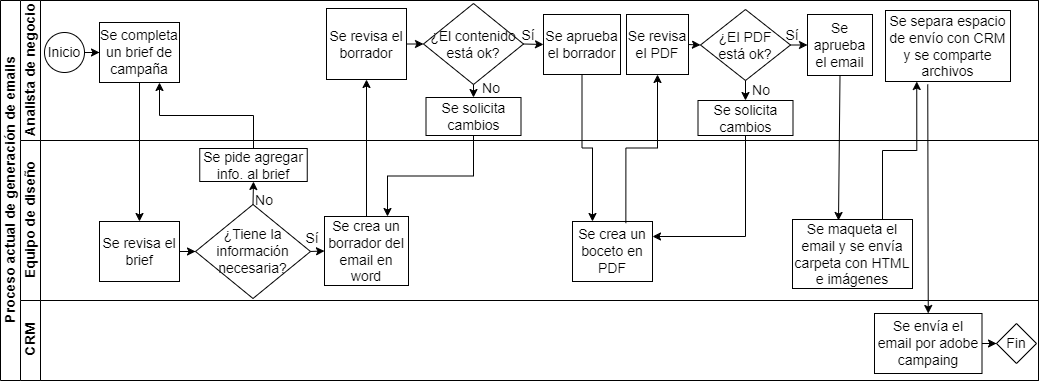
\includegraphics[width=\linewidth]{./Figures/Diagrama1_Creacion_Emails.png}
\caption{Proceso de creación de emails para clientes.}
\label{fig:procesoEmail}
\end{figure}
\end{landscape}

Como se puede observar, es un flujo largo que tiene muchas oportunidades de optimización. Este proceso inicia con la solicitud de creación de un email por parte de algún analista de negocio, el cual crea un \textit{brief} que es un documento que incluye el objetivo del correo, el contenido, público objetivo y otras instrucciones necesarias para su desarrollo. El equipo de diseño revisa este archivo y crea inicialmente un borrador del texto que se incluirá en el email. Tras su aprobación, recién inicia la maquetación del correo electrónico en HTML. Entre estos pasos, existen varias idas y vueltas entre ambos equipos para hacer correcciones en los bocetos que le toman al equipo de diseño varios días.

Sin embargo, gracias al avance de la inteligencia artificial (IA) generativa este proceso se puede reducir a unos pocos minutos, lo cual hace posible que las campañas comerciales y comunicación relacional sean enviadas a tiempo a los clientes. Además, se liberará de carga al equipo de diseño de tal forma que pueda enfocarse en actividades más creativas y que generen más valor a la organización. Esto implicará tanto ahorro de costos para la empresa como incremento en ventas gracias a la mejora en la comunicación comercial.

%----------------------------------------------------------------------------------------

\section{Objetivos y alcance}

El objetivo del trabajo propuesto es agilizar el proceso de creación de emails del Banco de Crédito del Perú y minimizar el esfuerzo humano mediante el uso de inteligencia artificial generativa. Estos correos deben crearse respetando los lineamientos de marca de la empresa, el estilo que corresponde a cada segmento de clientes del banco y deben aplicar correctamente la terminología bancaria.

\subsection{Alcance}

Este trabajo incluye una solución tecnológica en base a inteligencia artificial que pueda entender la información escrita en lenguaje natural brindada dentro de un \textit{brief} y, a partir de este, generar un email compuesto por texto e imágenes. Este email puede ser previsualizado por el usuario para permitir su revisión y aprobación. Una vez aprobado el diseño, el \textit{output} final que se comparte al solicitante es una carpeta con el archivo HTML y las imágenes necesarias.

Dentro de la solución brindada se incluyen las funcionalidades para poder pedir modificaciones sobre el documento HTML ya generado y poder adaptar el estilo a segmentos de clientes Bex y Enalta. Adicionalmente, se ha desarrollado una interfaz sencilla para que los usuarios no técnicos puedan usar el modelo.

El presente trabajo no incluye ninguna conexión directa con Adobe Campaign, que es la herramienta utilizada por la empresa para el envío de correos electrónicos. Tampoco está dentro del alcance la generación de emails para clientes corporativos del banco o correos con contenido de productos para empresas. Además, quedan pendientes las siguientes funcionalidades para futuros desarrollos: 

\begin{itemize}
    \item Poder incluir archivos \textit{GIF (Graphic Interchange Format)} dentro del email.
    \item Adaptar el estilo a segmentos de clientes Enalta y Banca Privada.
    \item Poder personalizar secciones del mail (como frases o imágenes) según \textit{clusters} de clientes específicos.
    \item Entre otras funcionalidades.
\end{itemize}

%----------------------------------------------------------------------------------------

\section{Estado del arte}

El desarrollo de la inteligencia artificial generativa ha sido rápido y disruptivo desde la publicación del influyente \textit{paper} \textit{Attention is All You Need} \citep{Vaswani2017} en 2017. En este se introdujo los transformadores, una arquitectura que ha revolucionado la forma en que las máquinas entienden y generan lenguaje humano y otros tipos de datos. Este método se basa exclusivamente en mecanismos de atención y prescinde de operaciones recurrentes en el procesamiento del lenguaje natural (NLP) \citep{Vaswani2017}. Esto permite a los modelos aprender relaciones complejas en datos de secuencia con mayor eficacia y eficiencia.

Gracias a eso, en 2018, casi simultáneamente, OpenAI y Google lanzaron GPT \citep{Radford2018} y BERT \citep{Devlin2018}, respectivamente. Estos modelos basados en transformadores mostraron capacidades superiores en muchas tareas de procesamiento del lenguaje natural. GPT, en particular, fue diseñado para la generación de texto \citep{Radford2018}, mientras que BERT se centró en mejorar la comprensión del contexto del lenguaje \citep{Devlin2018}.

Desde 2019, OpenAI ha seguido desarrollando y perfeccionando las versiones de GPT, que incluyen GPT-2 y GPT-3, este último lanzado en 2020. En sus inicios, estos modelos fueron utilizados principalmente por desarrolladores, ya que todavía no existía un producto diseñado para el público general. La versión de ChatGPT que se popularizó ampliamente, con una interfaz gráfica amigable para el usuario final, fue lanzada por OpenAI en noviembre de 2022. Esta versión fue específicamente optimizada para interacciones en forma de diálogo y diseñada para ser segura, fácil de usar y accesible para el uso masivo \citep{OpenAI2022ChatGPT}.

Los modelos de lenguaje de gran escala como GPT-3, lanzados durante este período, demostraron capacidades asombrosas como la generación de texto que puede ser indistinguible del escrito por humanos. El interés y la utilización de estos modelos se masificaron rápidamente, impulsados por su aplicación en una amplia gama de industrias, desde asistentes virtuales hasta herramientas de creación de contenido \citep{V7Labs2023}.

Entre las aplicaciones más interesantes de estos modelos están las herramientas de generación de código como GitHub Copilot \citep{GitHubCopilot2023}. Estas utilizan variantes de GPT-3 para ayudar a los desarrolladores a escribir código más rápido y con menos errores. Entre sus capacidades están autocompletar líneas de código, sugerir implementaciones completas de funciones y proporcionar ejemplos de código en tiempo real \citep{GitHubCopilot2023}. 

Por otro lado, en el campo de la generación de imágenes han surgido modelos basados en técnicas de difusión y GANs como DALL-E, Midjourney y Stability AI. Estos han mostrado cómo la IA puede crear imágenes artísticas y realistas a partir de descripciones textuales, revolucionando campos como el diseño gráfico y la moda \citep{BattleOfCreativity2024}.

Estos avances están cambiando la manera de trabajar, ya que permiten mayor eficiencia y nuevas formas de creatividad. La IA generativa sigue evolucionando, prometiendo aún más aplicaciones y mejoras en el futuro. Sin embargo, pese a sus impresionantes capacidades, no está exenta de desafíos y limitaciones. Algunos de los defectos más notables que se deben considerar al aplicarla en diversos desarrollos, son los siguientes \citep{TowardsAI2024}:

\begin{itemize}
    \item Sensibilidad a los \textit{prompts}: Los modelos generativos son altamente sensibles a la forma en que se estructuran los \textit{prompts} o instrucciones. Pequeñas variaciones en el texto pueden llevar a resultados significativamente diferentes. Esto requiere que los usuarios a menudo tengan que experimentar con diferentes formulaciones de \textit{prompts} para alcanzar el resultado deseado.
    \item Inconsistencias y errores fácticos: Los modelos pueden generar información que es inconsistente o incluso incorrecta. Esto es especialmente problemático en aplicaciones que requieren alta precisión factual, como en el ámbito médico o jurídico.
    \item Sesgos en los datos: Los modelos generativos aprenden de grandes volúmenes de datos y pueden heredar y perpetuar los sesgos presentes en esos datos. Esto puede resultar en respuestas sesgadas o injustas, particularmente en contextos sensibles como la contratación de personal o la toma de decisiones judiciales.
\end{itemize}

Para mitigar estos problemas, se utilizan varias herramientas y técnicas  \citep{TowardsAI2024}:

\begin{itemize}
    \item Ajuste fino y supervisión: ajustar modelos a conjuntos de datos específicos o supervisar y corregir sus salidas manualmente puede ayudar a mejorar la precisión y reducir errores.
    \item Desarrollo de \textit{prompts} efectivos: la creación de guías y herramientas para el desarrollo de \textit{prompts} más efectivos ayuda a los usuarios a interactuar de manera más eficiente con la IA y reduce la necesidad de múltiples intentos \citep{HatchWorks2024} \citep{arXiv2024Prompt}.
    \item Tecnologías de detección y mitigación de sesgos: se están desarrollando tecnologías específicas para detectar y mitigar sesgos en los modelos de IA, asegurando que los resultados sean más justos y equitativos.
    \item Pruebas rigurosas: implementar pruebas extensas en diversos escenarios puede ayudar a identificar y corregir errores antes de que los modelos se desplieguen en entornos de producción.
    \item Interfaz de usuario intuitiva: diseñar interfaces que guíen a los usuarios en la formulación de \textit{prompts} y en la interpretación de los resultados puede mejorar significativamente la experiencia del usuario y la calidad de los resultados generados.
\end{itemize}

En el presente trabajo se aplican estos nuevos modelos disruptivos para crear una solución al problema planteado y se toma en cuenta los desafíos que conlleva el uso de estas tecnologías para poder reducir lo máximo posible sus limitantes.
\chapter{Introducción específica} % Main chapter title

\label{Chapter2}

%----------------------------------------------------------------------------------------
%	SECTION 1
%----------------------------------------------------------------------------------------
En este capítulo se profundiza en conceptos de negocio que son importantes comprender para el desarrollo del trabajo. Adicionalmente se detallan los requerimientos y se brinda más detalle sobre los modelos de inteligencia artificial usados en la solución.

\section{Variables y reglas de negocio}
\label{sec:Negocio}

El Banco de Crédito del Perú es el banco más grande de su país con más de 11 millones de clientes y más de 17 mil empleados. Cuenta con diversas áreas de negocio repartidas según canales de atención, segmentos de clientes o productos. Por ejemplo, existen equipos de trabajo para canales alternativos como cajeros, otros para segmentos de clientes afluentes, y equipos para productos hipotecarios o de medios de pago, entre muchos otros. Cada uno de estos tiene analistas de negocio que se encargan de gestionar campañas comerciales o proyectos, muchos de los cuales exigen comunicaciones a los clientes. El email es uno de los primeros canales de comunicación que se eligen ya que no implica uso del presupuesto de área y es relativamente fácil de gestionar. Sin embargo, la mayoría de los pedidos de correos son derivados a un solo equipo de diseño, quien muchas veces debe priorizar y postergar algunos pedidos por falta de capacidad.

El equipo de diseño desarrolla los emails en base a \textit{briefs}. En el caso de campañas grandes que exigen varios canales de comunicación y una estrategia más compleja, se tienen \textit{briefs} más extensos. Pero en general, para correos tácticos, se utiliza un \textit{mini-brief} que incluye estas preguntas:

\begin{enumerate}
    \item Objetivo de la campaña:
    \item ¿Quién es nuestro público objetivo?
    \item ¿Qué queremos decirles?
    \item ¿A qué segmentos va dirigido? Si incluye ENALTA, confirmar la firma de quién irá en el mail.
    \item Tipo de Piezas y mandatorios
\end{enumerate}

Las tres primeras preguntas ayudan a dar contexto sobre qué se quiere lograr con la comunicación, cómo adaptarla según el público al que va dirigida y detalla el contenido del email. La cuarta pregunta pide especificar el segmento del cliente.

Dentro del banco, existen diferentes segmentos de clientes personas naturales que se definen principalmente en base a los ingresos y patrimonio de los estos. De menos a más ingresos, estos son los segmentos: 
\begin{itemize}
    \item Consumo
    \item Banca Exclusiva (BEX)
    \item Enalta
    \item Privada
\end{itemize}

Cada segmento tiene colores y diseños de emails ligeramente diferentes. En específico, Enalta y Privada tienen incluso sus propios logos. Adicionalmente, los cierres de los correos cambian. En Consumo, el cierre es más general y se derivan las consultas a canales de atención masivos. Para el resto de los segmentos, los cierres derivan las consultas a los funcionarios asignados a cada cliente en específico, por lo que en el código HTML se incluyen campos personalizables para estos casos. Para el alcance del presente trabajo solo se están considerando los segmentos Comsumo y BEX, ya que abarcan la mayoría de clientes. 

En las figuras~\ref{fig:EjConsumo} y~\ref{fig:EjBEX} se pueden visualizar ejemplos de las variantes de emails de una misma campaña para estos dos segmentos. Adicionalmente, también podemos ver un análisis inicial que se ha realizado de las partes que componen un correo, lo cual será crucial para el desarrollo de la solución. Como se puede notar, La cabecera y el cierre son los que más variaciones tienen entre Consumo y BEX. Además, a veces también se presentan cambios en el color del texto para resaltar frases importantes.

Otra sección del correo que es importante considerar son los Términos y Condiciones (T\&C) y los legales. Los T\&C son opcionales y los analistas de negocio los tienen que compartir textualmente en el \textit{brief}. Estos se incluyen sin ninguna modificación en el email, ya que han sido revisados previamente por el área de legal. Adicionalmente, existe un texto genérico que se incluye en todos los emails del banco (los dos últimos párrafos). Este legal genérico no es necesario mencionarlo en el \textit{brief} ya que el equipo de diseño siempre lo incluye en los correos como parte de los lineamientos que tiene. 

Por último, para comunicaciones de productos que tienen asociadas tasas, es necesario incluir tasas referenciales en el legal. La tasa especificada puede ser tasa de costo efectiva anual (TCEA) para productos activos (aquellos que involucran que el banco preste dinero al cliente), o tasa de rendimiento efectiva anual (TREA) para productos pasivos (aquellos en los que el cliente deja su dinero en custodia del banco). Tanto la tasa como su descripción también deben ser brindadas por el analista de negocios en el \textit{brief}.

\cleardoublepage
\begin{figure}[!htpb]
     \centering
     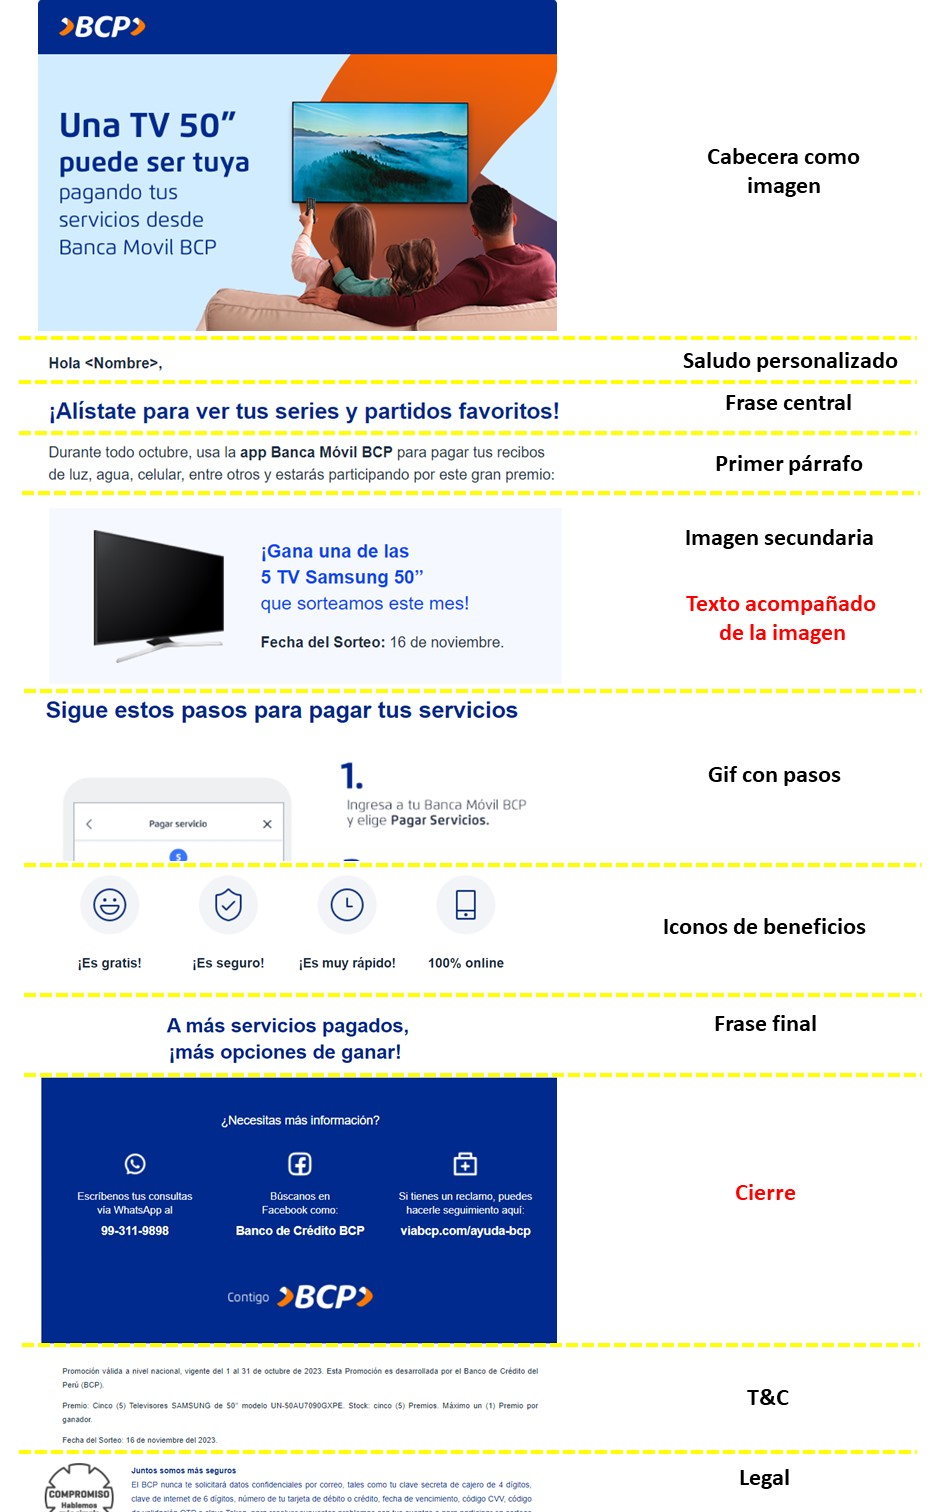
\includegraphics[width=0.8\textwidth]{./Figures/ejemplo_Consumo}
    \caption{Ejemplo de email para Consumo}
    \label{fig:EjConsumo}
\end{figure}

\begin{figure}[!htpb]
     \centering
     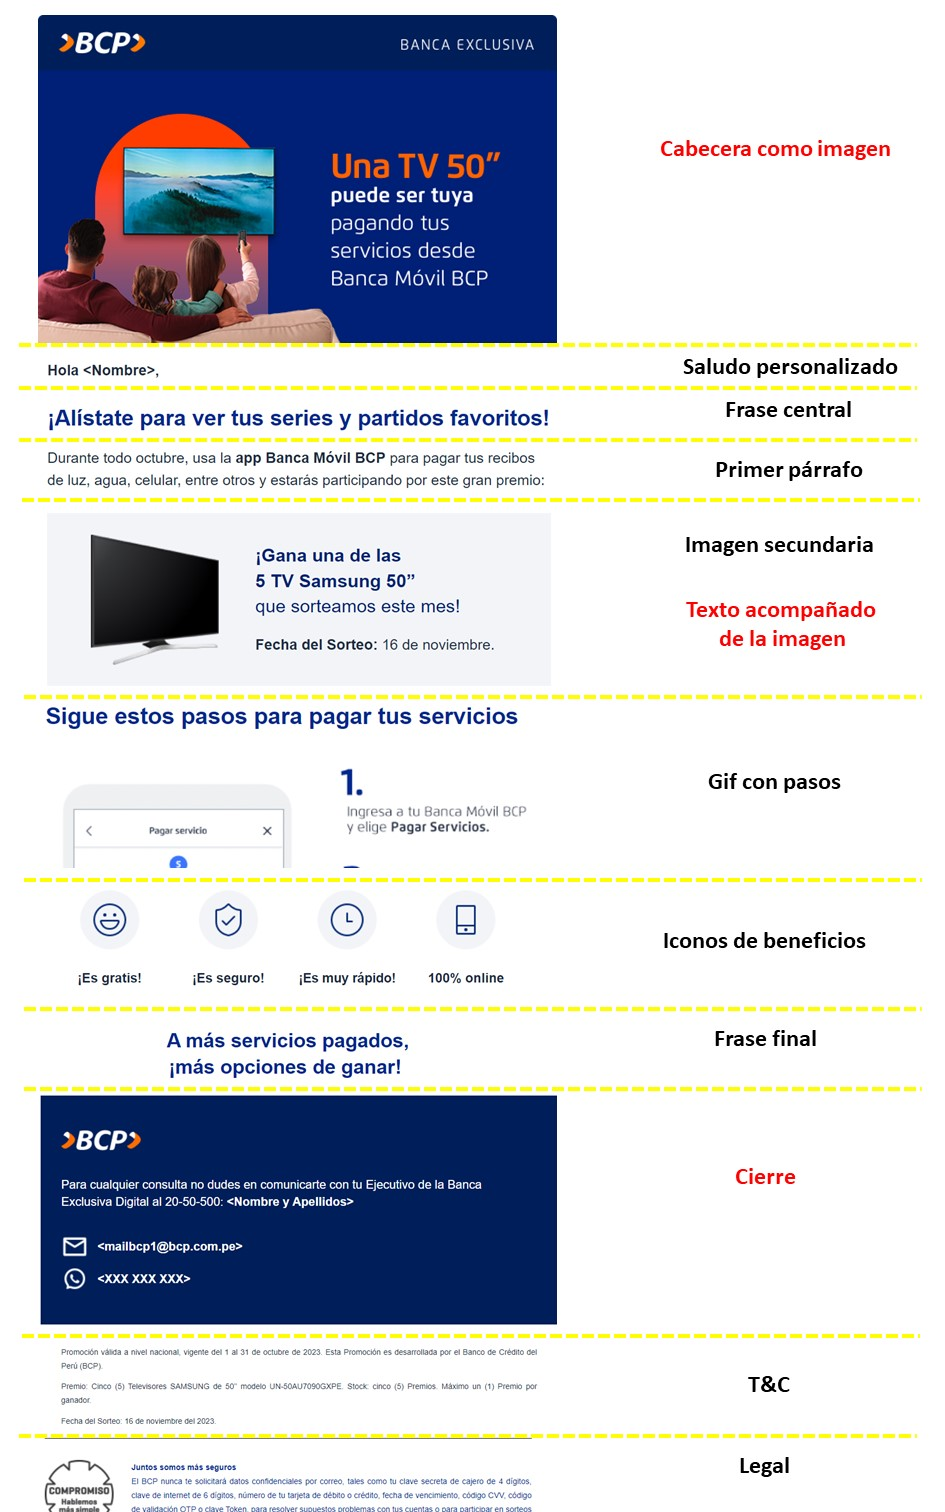
\includegraphics[width=0.8\textwidth]{./Figures/ejemplo_BEX}
     \caption{Ejemplo de email para BEX}
     \label{fig:EjBEX}
\end{figure}


\section{Requerimientos}

Los requerimientos que se han considerado al momento de desarrollar el presente trabajo son los siguientes:

\begin{enumerate}
	\item Requerimientos funcionales
		\begin{enumerate}
			\item El sistema debe generar un boceto de email según lo información brindada en un \textit{brief} que incluye: 1) Objetivo de la campaña 2) Público objetivo 3) Mensaje que se desea comunicar.
			\item El formato final del proceso es un archivo index.html con una carpeta ``img"  que contenga las imágenes necesarias para el mail. Este formato es compatible con Adobe Campaign.
			\item Se debe generar un output intermedio que permita al usuario revisar el contenido del email antes de su versión final.
			\item El email generado debe cumplir con los lineamientos de diseño de correos de la empresa, considerando que el formato cambia según los segmentos de clientes.
		\end{enumerate}
	\item Requerimientos de confidencialidad y seguridad
		\begin{enumerate}
			\item La información de la empresa brindada para entrenar el modelo no debe ser compartida con terceras empresas.
			\item La información que se comparte al modelo mediante los \textit{briefs} no debe contener datos de alta criticidad de clientes o personas (número de documento, nombres, datos de contacto, entre otros).
		\end{enumerate}
	\item Requerimientos de la interfaz (opcional)
		\begin{enumerate}
			\item El modelo debe poder ser utilizado por usuarios no técnicos pertenecientes a equipos de diseño y marketing.
		\end{enumerate}
\end{enumerate}

\section{Modelos de generación de texto utilizados}

El Procesamiento del Lenguaje Natural (PLN) es un campo de la inteligencia artificial que se encarga de la interacción entre las computadoras y el lenguaje humano. Este campo abarca el desarrollo de algoritmos y sistemas que permiten a las máquinas comprender, interpretar y generar lenguaje humano de manera efectiva, facilitando aplicaciones como la traducción automática, el análisis de sentimientos, los chatbots y la síntesis de texto \cite{jurafsky2021}.

Los Modelos de Lenguaje a Gran Escala (LLMs, por sus siglas en inglés) son modelos de aprendizaje profundo entrenados en grandes cantidades de texto para predecir la probabilidad de secuencias de palabras. Se les llama "grandes" por la enorme cantidad de parámetros que manejan, lo cual les permite captar complejidades y matices del lenguaje natural \cite{vaswani2017}.

Estos modelos han sido entrenados utilizando técnicas de pre-entrenamiento en grandes corpus de texto, lo que les permite aprender patrones y estructuras del lenguaje. Utilizan tokens, que son unidades básicas de texto (como palabras o subpalabras), para procesar y generar lenguaje. Actualmente, los LLMs se utilizan para una variedad de tareas como la generación de texto, la traducción automática, la respuesta a preguntas y la síntesis de texto \cite{vaswani2017}.

Entre los LLMs más destacados disponibles actualmente se encuentran GPT-4, Claude, GPT-3.5, Vicuna, y LLaMA, entre otros. Algunos de estos modelos son de código abierto, como Vicuna y LLaMA, mientras que otros son privados, como GPT-4. Un estudio reciente comparó estos modelos utilizando tanto jueces humanos como las propias LLMs para determinar cuál es mejor en diversas tareas. En este estudio, GPT-4 fue uno de los modelos ganadores, mostrando un rendimiento superior en varias métricas \cite{zheng2023judging}. La figura a continuación muestra la tasa de victorias promedio de nueve modelos bajo diferentes jueces en Chatbot Arena:

\begin{figure}[h]
  \centering
  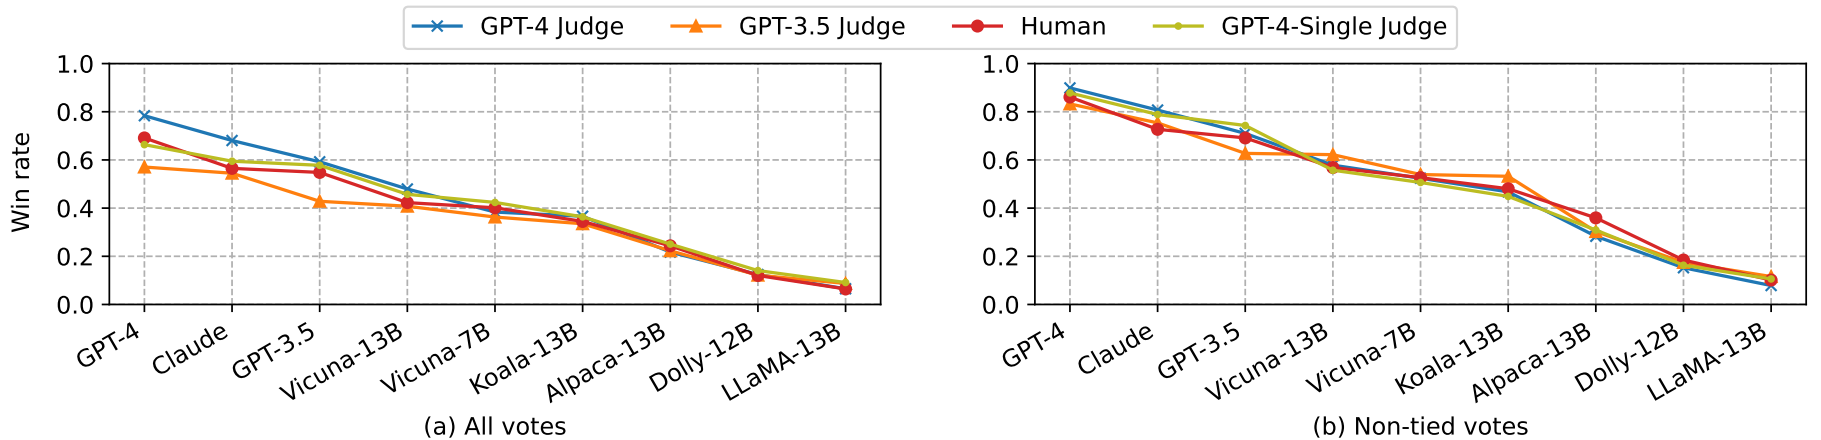
\includegraphics[width=\linewidth]{./Figures/comparacion_LLMs.png}
  \caption{Tasa promedio de victorias de nueve modelos bajo diferentes jueces. Primer gráfico considerando todos los votos y segundo, solo los votos sin empates\cite{zheng2023judging}.}
\end{figure}

Varias LLMs privadas están disponibles para su uso mediante API. Por ejemplo, OpenAI ofrece una API que permite acceder a modelos como GPT-4o, GPT-4 y GPT-3, entre otros. Estas API ofrecen funcionalidades como el modo JSON para estructurar las respuestas. El uso de estas API se cobra en función de los tokens de entrada y salida procesados. En nuestro proyecto, decidimos usar GPT-4o, ya que es un modelo más reciente que GPT-4 y resulta más económico \cite{openai}.

LangChain es un marco de trabajo diseñado para facilitar el desarrollo de aplicaciones que utilizan LLMs. Es útil porque proporciona herramientas y abstracciones para conectar modelos de lenguaje con otras fuentes de datos y sistemas, permitiendo la creación de flujos de trabajo complejos y personalizados. Las cadenas en LangChain funcionan conectando diferentes componentes que procesan y transforman datos en pasos secuenciales \cite{langchain}.

Además, mediante LangChain también se pueden crear agentes de inteligencia artificial. Un agente AI es un sistema que puede percibir su entorno y tomar acciones para alcanzar objetivos específicos. En LangChain, se pueden definir herramientas (tools) que los agentes pueden utilizar para ejecutar funciones dentro de las aplicaciones, permitiendo una interacción más rica y compleja con los usuarios \cite{langchain}.

\section{Modelos de generación de imágenes utilizados} 
\chapter{Diseño e implementación} % Main chapter title

\label{Chapter3} % Change X to a consecutive number; for referencing this chapter elsewhere, use \ref{ChapterX}

\definecolor{mygreen}{rgb}{0,0.6,0}
\definecolor{mygray}{rgb}{0.5,0.5,0.5}
\definecolor{mymauve}{rgb}{0.58,0,0.82}

%%%%%%%%%%%%%%%%%%%%%%%%%%%%%%%%%%%%%%%%%%%%%%%%%%%%%%%%%%%%%%%%%%%%%%%%%%%%%
% parámetros para configurar el formato del código en los entornos lstlisting
%%%%%%%%%%%%%%%%%%%%%%%%%%%%%%%%%%%%%%%%%%%%%%%%%%%%%%%%%%%%%%%%%%%%%%%%%%%%%
\lstset{ %
  backgroundcolor=\color{white},   % choose the background color; you must add \usepackage{color} or \usepackage{xcolor}
  basicstyle=\footnotesize\ttfamily,        % the size of the fonts that are used for the code
  breakatwhitespace=false,         % sets if automatic breaks should only happen at whitespace
  breaklines=true,                 % sets automatic line breaking
  captionpos=b,                    % sets the caption-position to bottom
  commentstyle=\color{mygreen},    % comment style
  deletekeywords={...},            % if you want to delete keywords from the given language
  %escapeinside={\%*}{*)},          % if you want to add LaTeX within your code
  %extendedchars=true,              % lets you use non-ASCII characters; for 8-bits encodings only, does not work with UTF-8
  %frame=single,	                % adds a frame around the code
  keepspaces=true,                 % keeps spaces in text, useful for keeping indentation of code (possibly needs columns=flexible)
  keywordstyle=\color{blue},       % keyword style
  language=Python,                 % the language of the code
  %otherkeywords={*,...},           % if you want to add more keywords to the set
  numbers=left,                    % where to put the line-numbers; possible values are (none, left, right)
  numbersep=5pt,                   % how far the line-numbers are from the code
  numberstyle=\tiny\color{mygray}, % the style that is used for the line-numbers
  rulecolor=\color{black},         % if not set, the frame-color may be changed on line-breaks within not-black text (e.g. comments (green here))
  showspaces=false,                % show spaces everywhere adding particular underscores; it overrides 'showstringspaces'
  showstringspaces=false,          % underline spaces within strings only
  showtabs=false,                  % show tabs within strings adding particular underscores
  stepnumber=1,                    % the step between two line-numbers. If it's 1, each line will be numbered
  stringstyle=\color{mymauve},     % string literal style
  tabsize=2,	                   % sets default tabsize to 2 spaces
  title=\lstname,                  % show the filename of files included with \lstinputlisting; also try caption instead of title
  morecomment=[s]{"""}{"""},
  morekeywords={self,as,assert,nonlocal,with,yield,self,True,False,None,,object,type,isinstance,copy,deepcopy,zip,enumerate,reversed,list,set,len,dict,tuple,range,xrange,append,execfile,real,imag,reduce,str,repr,ode,fsolve,sqrt,exp,sin,cos,arctan,arctan2,arccos,pi, array,norm,solve,dot,arange,isscalar,max,sum,flatten,shape,reshape,find,any,all,abs,plot,linspace,legend,quad,polyval,polyfit,hstack,concatenate,vstack,column_stack,empty,zeros,ones,rand,vander,grid,pcolor,eig,eigs,eigvals,svd,qr,tan,det,logspace,roll,min,mean,cumsum,cumprod,diff,vectorize,lstsq,cla,eye,xlabel,ylabel,squeeze},
  inputencoding=utf8,              % usa UTF-8 para interpretar el código
  literate=%
    {á}{{\'a}}1 {é}{{\'e}}1 {í}{{\'i}}1 {ó}{{\'o}}1 {ú}{{\'u}}1
    {Á}{{\'A}}1 {É}{{\'E}}1 {Í}{{\'I}}1 {Ó}{{\'O}}1 {Ú}{{\'U}}1
    {ñ}{{\~n}}1 {Ñ}{{\~N}}1 {¿}{{\textquestiondown}}1 {¡}{{\textexclamdown}}1
}

%----------------------------------------------------------------------------------------
%	INTRODUCCIÓN AL CAPÍTULO
%----------------------------------------------------------------------------------------

En este capítulo se explica cómo se han utilizado los modelos y herramientas de inteligencia artificial descritos en los capítulos anteriores junto con otras técnicas de programación para crear una aplicación que permite generar tanto el contenido como las imágenes de un email de forma automática. Se detallan desde los primeros intentos en explorar las posibles soluciones, hasta la forma como se terminaron construyendo los módulos de generación de texto, imagen y la interfaz gráfica.

%----------------------------------------------------------------------------------------
%	SECTION 1
%----------------------------------------------------------------------------------------

\section{Aproximación inicial a la solución y diseño de plantillas}

La ideación de la solución comenzó con experimentos básicos en los que se le pedía a ChatGPT construir emails en HTML brindándole una plantilla a través de la interfaz de OpenAI. El propósito de estos experimentos era probar qué tan bueno podía ser un gran modelo de lenguaje al crear un email a partir de una plantilla. En la figura~\ref{fig:PruebaChatGPT} se puede ver el resultado (ignorar para este caso la imagen, ya que únicamente se estaba testeando la generación de texto). En el lado izquierdo se puede observar cómo se ve la plantilla brindada a ChatGPT con un mensaje inventado que debía ser modificado por el modelo. Cabe resaltar que se le dio la plantilla como código HTML. Posteriormente, se le dio la siguiente instrucción:

\begin{quote}
``Quiero que mantengas las imágenes, pero cambia el contenido del email. Cámbialo para que sea un campaña de venta de tarjeta de crédito: Adquiere tu tarjeta de crédito Visa Signature con S/ 20 000 de línea de crédito. Tendrás múltiples beneficios (colocar los beneficios en viñetas): descuentos en restaurantes, pases a las salas vip de aeropuertos, cuotas sin intereses, tasa preferencial de 20\%.''
\end{quote}

Como se observa en el resultado 1 de la figura~\ref{fig:PruebaChatGPT}, el modelo cambia correctamente el mensaje y brinda un título y párrafos coherentes con lo solicitado. Sin embargo no termina de generar todo el contenido por la gran extensión de la parte legal de la plantilla. En vez de brindar el email completo, el modelo colocó este mensaje dentro del código: \texttt{<!-- Resto del contenido... -->}. 

Se le pidió al modelo brindar el resto del código que debía ser colocado en vez de ese mensaje y generó código que se tuvo que copiar y pegar manualmente para obtener el resultado 2 de la figura~\ref{fig:PruebaChatGPT}. En esta segunda iteración se logró un email más completo. Sin embargo, el modelo colocó un texto legal más resumido, inventó un nombre para la página de Facebook de la compañía distinto al brindado en la plantilla y también creó un URL ficticio de la web oficial.

\begin{figure}[!htpb]
     \centering
     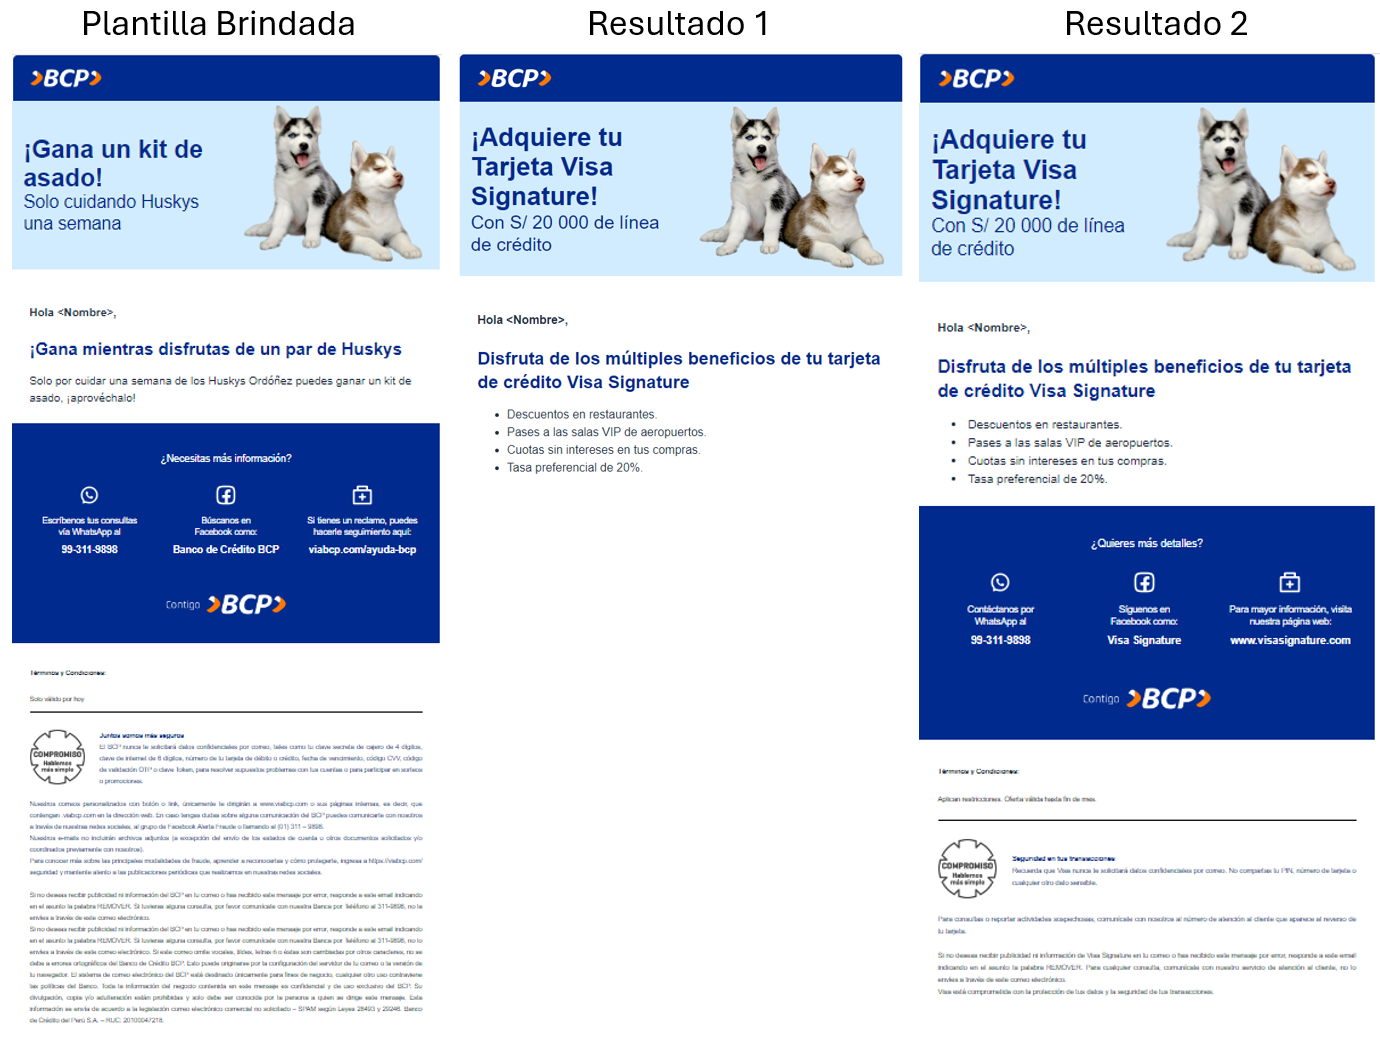
\includegraphics[width=1\textwidth]{./Figures/Prueba_Inicial_Chatgpt.png}
    \caption{Prueba realizada con ChatGPT.}
    \label{fig:PruebaChatGPT}
\end{figure}

Con esta experiencia se sacaron varias conclusiones. Una de ellas es que los LLMs sí son capaces de entender HTML y modificar su contenido coherentemente, pero tienden a limitar la cantidad de \textit{tokens} que brindan como \textit{output}, por lo que pueden arrojar emails incompletos. 

Adicionalmente, hay partes como el legal o la web de la empresa, que ya están definidos y no se necesita que un LLM las modifique. Incluso su modificación es perjudicial. Darle la oportunidad al LLM de que edite un correo completo incrementa la posibilidad de que se cambien partes del email que no se deben alterar como los colores de marca, la maquetación, los datos de contacto, entre otros detalles.

Por otro lado, el costo de usar un LLM está relacionado a la cantidad de \textit{tokens} de \textit{input} y \textit{output}, por lo que brindarle una plantilla con todo el texto legal y pedirle que retorne el mismo texto sin modificaciones no es eficiente en términos de procesamiento ni de costos.

Este análisis inicial condujo a la decisión de optar por una solución más estructurada mediante la creación de clases y funciones que utilicen código HTML de plantillas predefinidas sin necesidad de que el gran modelo de lenguaje las tenga que conocer a detalle. Lo único que es necesario que el LLM genere es el contenido variable del email, que posteriormente es insertado en las plantillas.

Para lograr este planteamiento, la primera tarea consistió en comprender la estructura de un email modelo proporcionado por la empresa e identificar todos los elementos que lo componen. Entre ellos están los siguientes: la cabecera, el cuerpo principal, el cierre y la sección legal. El detalle de la estructura de un email modelo se presentó en el capítulo anterior en las figuras~\ref{fig:EjConsumo} y~\ref{fig:EjBEX}.

Poder separar los elementos del email permitió identificar cuáles se deben modificar de los que no. Los elementos que no se modifican se dejan como parte del código de las plantillas, mientras que las partes que sí cambian son manejadas como \textit{inputs} para la creación de clases. 

Se crearon 2 objetos principales que son los encargados de recibir los \textit{inputs} del contenido del email e insertarlos dentro de las plantillas para obtener el HTML final. A estos objetos se los denominó \texttt{Email\_html} y \texttt{Contenido\_principal}. A su vez, se crearon clases secundarias para manejar el contenido que se puede agregar al email de forma opcional: \texttt{Contenido\_extra}, \texttt{Legal\_extra}, \\ \texttt{Seccion\_iconos}, \texttt{Recuadro\_premio} y \texttt{Recuadro\_lista}.

En la figura~\ref{fig:Diagrama_clases} se encuentra un diagrama que ayuda a entender mejor la relación entre estas clases y los elementos que contiene cada una. Existen clases que son \textit{inputs} de otras más generales. El objeto que engloba a todas y cuya instancia representa un email completo con todos sus elementos es la clase \texttt{Email\_html}. 


\begin{figure}[!htpb]
    \centering
    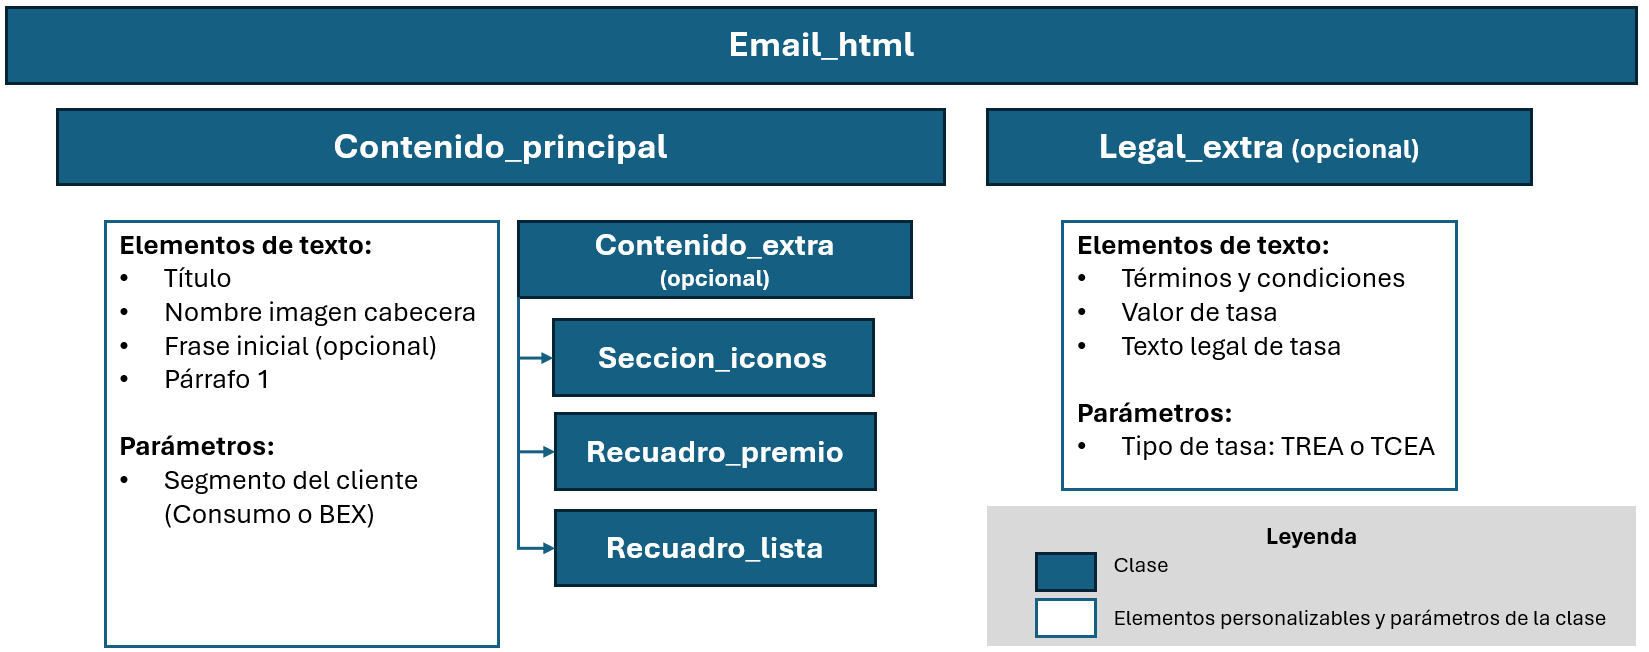
\includegraphics[width=0.95\linewidth]{Figures/Diagrama_clases.png}
    \caption{Diagrama de clases y sus elementos.}
    \label{fig:Diagrama_clases}
\end{figure}

En la figura~\ref{fig:DefinicionClase} se puede observar la estructura general que se ha seguido para definir una clase.

\begin{figure}[!htpb]
    \centering
    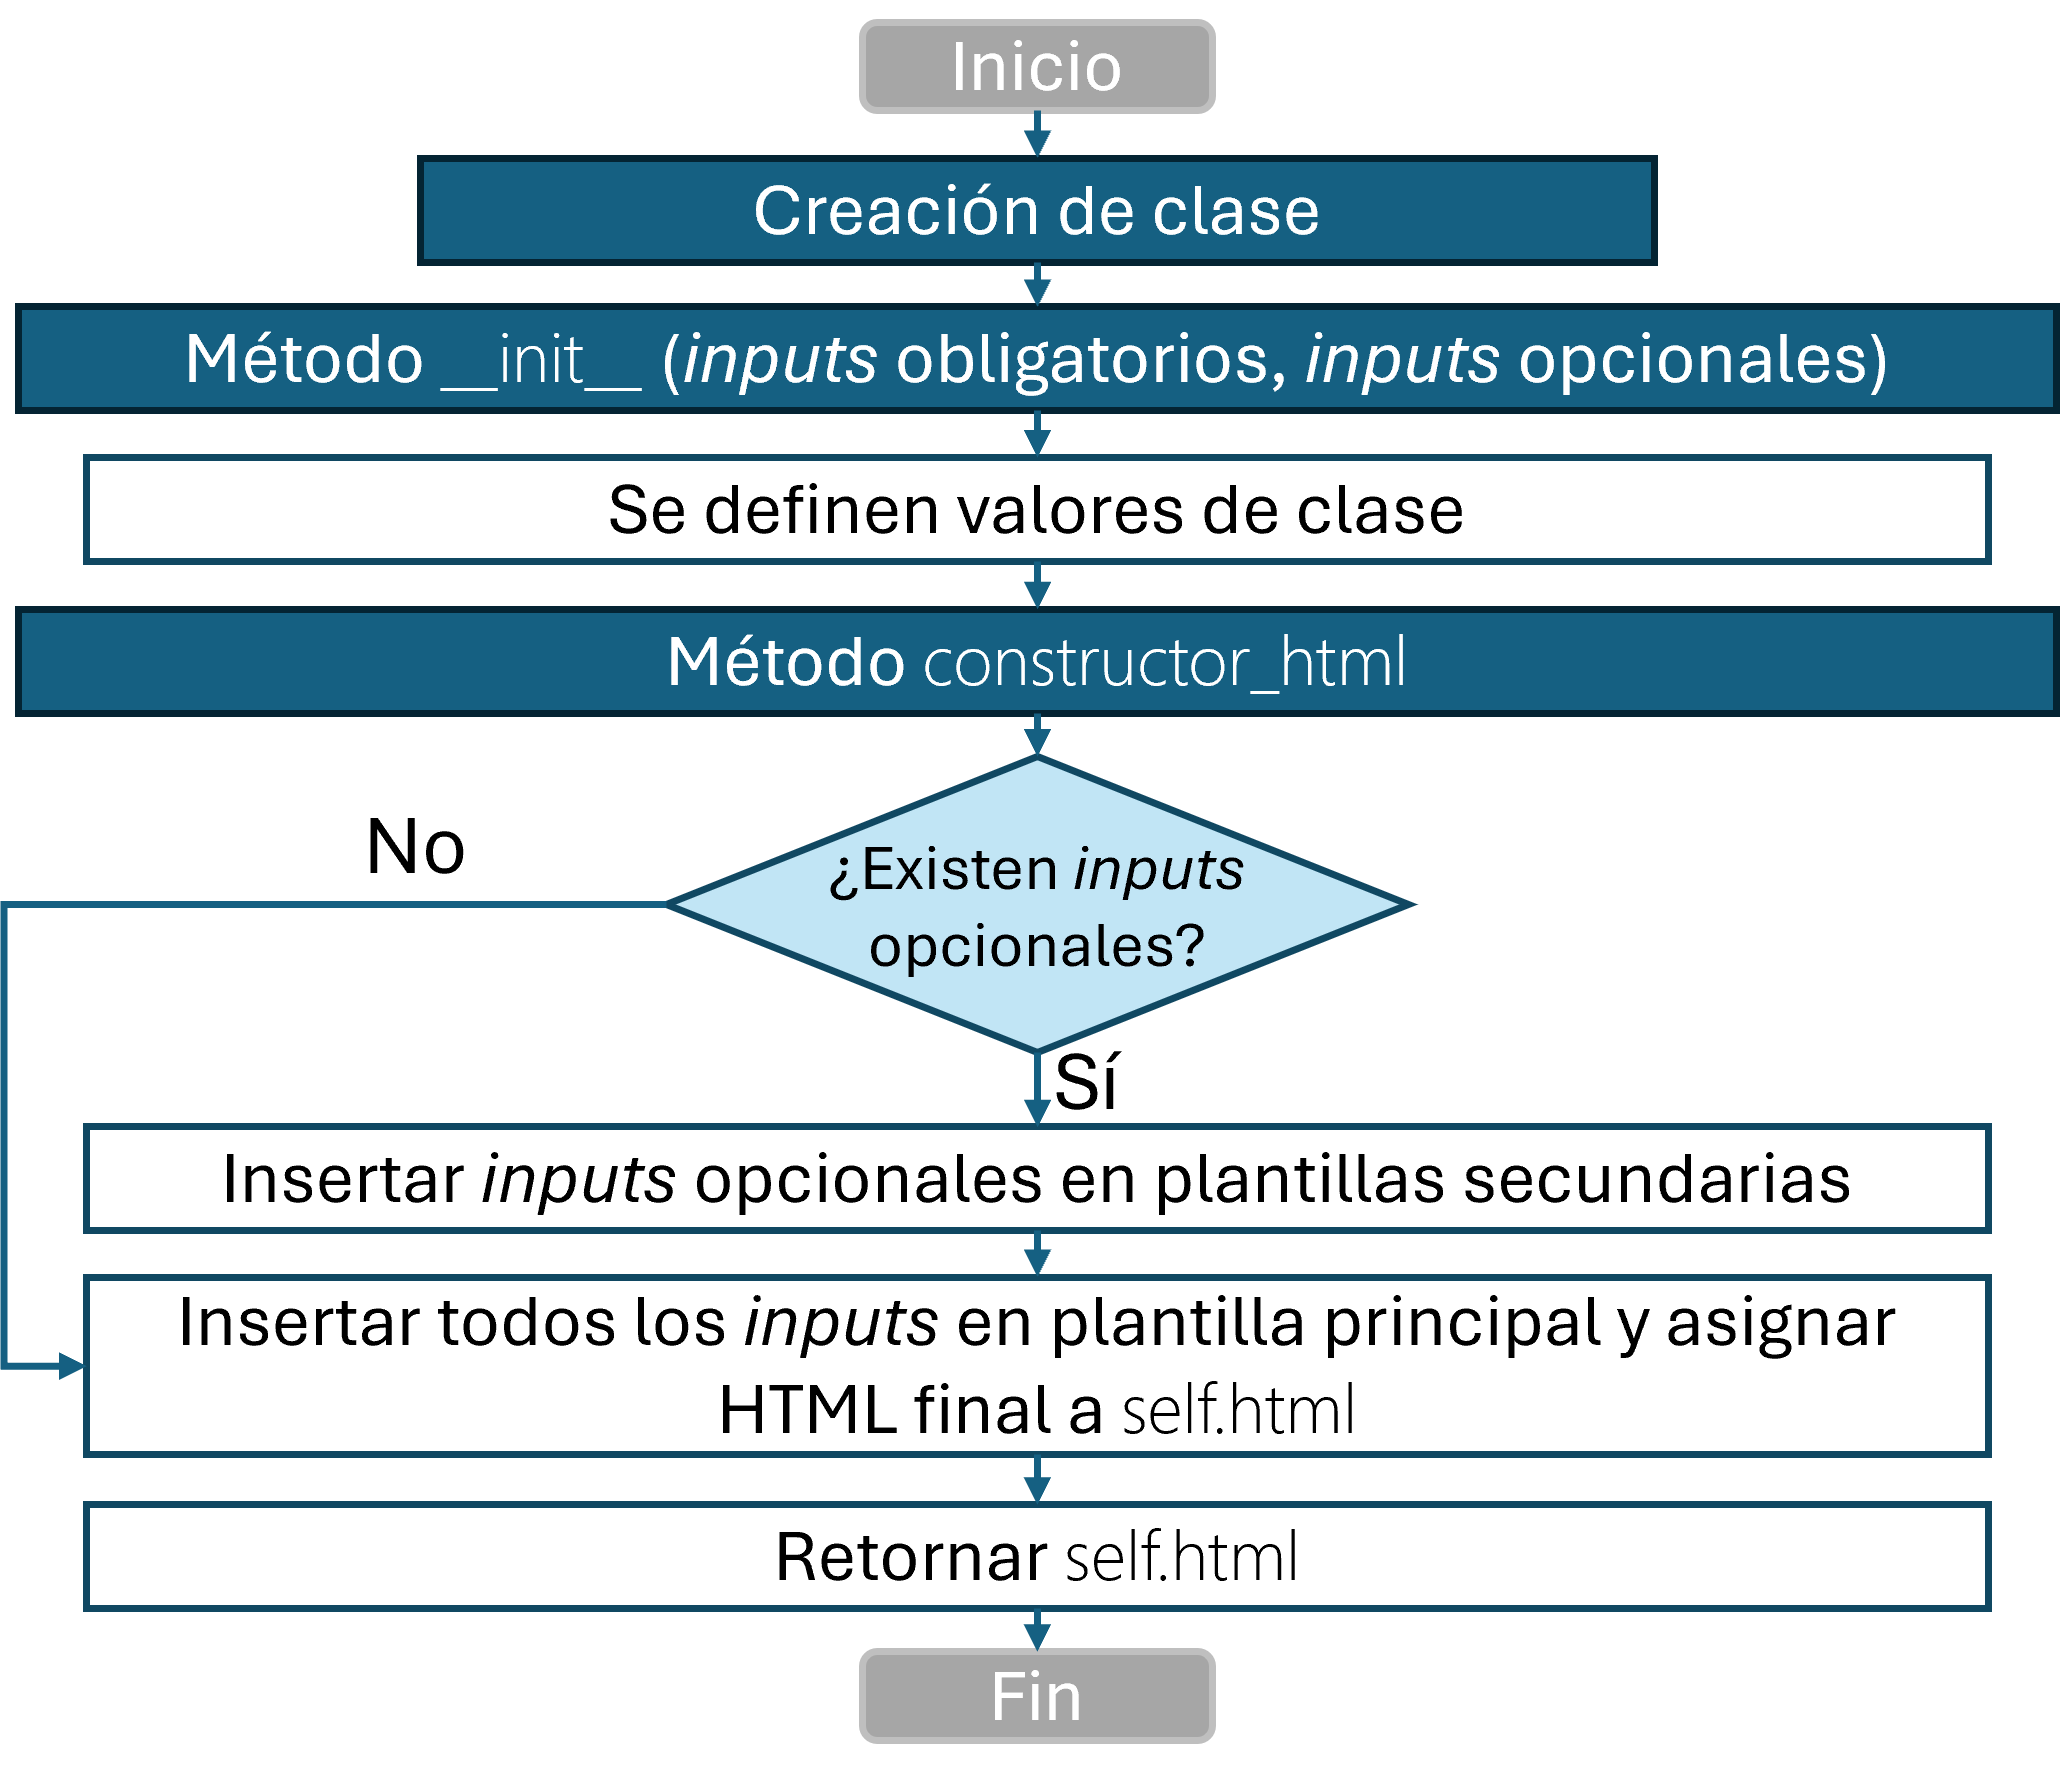
\includegraphics[width=0.7\linewidth]{Figures/Flujo_creacion_clase.png}
    \caption{Flujo de la creación de una clase HTML.}
    \label{fig:DefinicionClase}
\end{figure}

Como se muestra en el diagrama, al inicializar la clase se le comparten ciertos parámetros que son obligatorios y otros que son opcionales. Por ejemplo, en el caso de la clase \texttt{Contenido\_principal}  los obligatorios son \texttt{segmento\_cliente}, \\ \texttt{img\_cabecera}, \texttt{titulo\_1}, \texttt{titulo\_2} y \texttt{parrafo\_1}. Estos son los mínimos elementos necesarios para generar un email coherente. En específico, el parámetro \texttt{segmento\_cliente} es el que indica si se usará la plantilla de un email para clientes BEX o Consumo. Por otro lado, los parámetros opcionales para esta clase son la \texttt{frase\_inicial} y una instancia de la clase \texttt{Contenido\_extra}.

Una vez que se inicializa la clase, se utiliza el método \texttt{constructor\_html} para poder llamar a las plantillas correspondientes e insertarles el contenido. Todas las plantillas utilizan \textit{string format} para poder insertar contenido de variables dentro del texto y están definidas en el módulo \texttt{mod\_string\_format.py}. Específicamente la clase \texttt{Contenido\_principal} utiliza las siguientes plantillas: \\ \texttt{contenido\_consumo}, \texttt{contenido\_bex}, \texttt{frase\_inicial} . 

Con la creación de estas plantillas y clases que se encargan de armar el HTML de forma más ordenada, el siguiente paso fue conseguir que el gran modelo de lenguaje pueda trabajar con estas clases y brindarles los \textit{inputs} adecuados para que el email pueda ser generado. Esta parte del desarrollo se explica en la siguiente sección.

%-------------------------------------------------------------------------------------------------------------
%-------------------------------------------------------------------------------------------------------------

\section{Generación del contenido del email con LLMs}

Para lograr que el modelo de lenguaje pueda utilizar las clases creadas se decidió optar por crear un agente LLM. Como se explicó en la sección~\ref{sec:LagchainAgentes}, los agentes tienen la particularidad de que se les pueden brindar herramientas (\textit{tools}) para que realicen acciones y ejecuten código, no solo generar texto, que era lo que se necesitaba para este proyecto. El agente puede ejecutar una función que reciba como parámetros los \textit{inputs} del contenido del email y los utilice para crear las instancias de clases necesarias.

Para la creación del agente basado en un modelo de lenguaje, se decidió utilizar LangChain \cite{langchain}. A través de LangChain, se configuró el acceso a la API de OpenAI que permite realizar solicitudes a grandes modelos de lenguaje como GPT4o-mini. Además, LangChain ya proporciona plantillas y estructuras para poder generar agentes con \textit{tools} personalizados. Para este trabajo, se decidió utilizar un agente ReAct \cite{yao2022react}, que está instruido para razonar antes de realizar una acción. Seguir esta secuencia lógica le permite al LLM detenerse a analizar qué \textit{tool} usar y cómo usarlo antes de ejecutar cualquier función.

\subsection{Creación de la función create\_email}

La función \texttt{create\_email} es la que se le asignó al agente LLM como \textit{tool} para que ejecute y es importante porque es la conexión entre el modelo y las clases y plantillas creadas. Inicialmente se hicieron pruebas creando una función que recibía varios parámetros (uno por elemento del email), pero el modelo de agente ReAct que se estaba usando fallaba al tener que brindar más de un parámetro. Así que se optó por crear una función con un solo parámetro de entrada: un texto en formato JSON que contenga todos los elementos del email.

Este texto se convierte a JSON dentro de la función y sus elementos se van utilizando para inicializar las clases correspondientes. El formato JSON resultó ser bastante conveniente ya que permite decidir qué elementos enviar y cuáles no, algo útil al momento de trabajar con los \textit{inputs} opcionales del email. Para el manejo de estos campos opcionales, se incluyó dentro de la función validaciones para adaptar la inicialización de las clases dependiendo si se envían estos campos o no. En la figura~\ref{fig:createEmail} se puede ver la estructura de la función \texttt{create\_email} con más detalle.

\begin{figure}[!htpb]
    \centering
    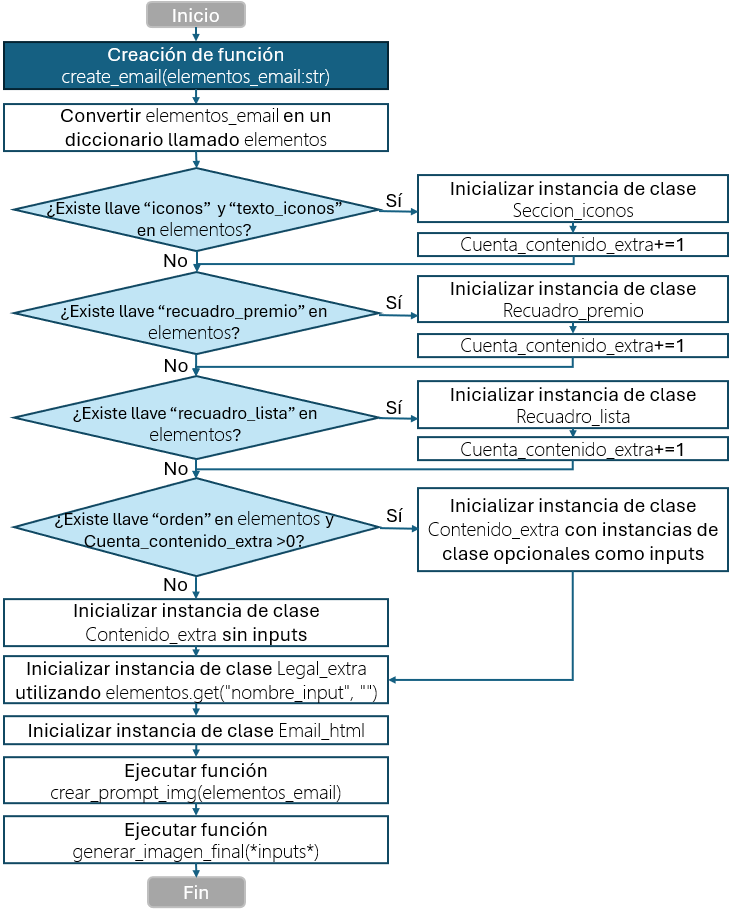
\includegraphics[width=1\linewidth]{Figures/Flujo_create_email.png}
    \caption{Flujo de la función \texttt{create\_email}.}
    \label{fig:createEmail}
\end{figure}

Como se puede observar, la variable \texttt{elementos} es un diccionario que se crea a partir del JSON y es la que contiene todos los \textit{inputs} del contenido del email. Existen algunos elementos como \texttt{iconos} o \texttt{tcea\_trea} que son opcionales y se usan estructuras \texttt{if} o el método \texttt{.get} para validar si se enviaron. Al usar \texttt{.get}, en caso de que no se encuentren, se deja su valor como un \texttt{string} vacío, que no afecta el contenido del HTML al insertarse.

La función \texttt{create\_email} contiene también un llamado a otras funciones que generan la imagen de cabecera. Estas serán explicadas en la sección~\ref{sec:GeneracionImg}. Por el momento, lo importante es comentar que dentro del JSON de \textit{input} ya se recibe el nombre de la imagen de cabecera que se incrusta en el HTML. Este se pasa como \textit{input} a la función \texttt{generar\_imagen\_final} para que la imagen a ser generada sea guardada con ese mismo nombre.


\subsection{Creación de las plantillas del \textit{prompt}}

Una parte fundamental al momento de trabajar con grandes modelos de lenguaje es explicarles en detalle lo que se espera que hagan. Esto se logra creando buenas plantillas de \textit{prompts}. Cuando se crea un agente, se necesita más de un \textit{prompt}. Existe uno principal, que es el que le explica al modelo cuál será su rol y sus tareas principales. Luego existe otro por cada \textit{tool} que se le brinde, que explica para qué sirve la herramienta y cómo utilizarla correctamente.

A continuación, se presenta el \textit{prompt} principal del agente que detalla el rol o tarea general que debe cumplir. También es aquí donde se inserta el contenido del email que brinda el usuario.

\begin{quote}
``Ayuda a crear el html para un email considerando este contenido y especificaciones:

Contenido del email: \texttt{\{contenido\}}

Si recibes un error, intenta nuevamente asegurándote de enviar el json en el formato correcto.''
\end{quote}

El segundo \textit{prompt} creado es el del \textit{tool} que explica cómo usar la función \\ \texttt{create\_email}. Este es mucho más extenso porque da bastante detalle sobre cómo estructurar el contenido del email en cada llave del JSON. En el apéndice~\ref{AppendixA} se encuentra el \textit{prompt} completo, pero se puede resumir en los siguientes pasos:

\begin{itemize}
    \item Se explica para qué sirve la herramienta \texttt{create\_email}.
    \item Se informa que el \textit{input} de la función es un texto en formato JSON.
    \item Se enlistan los elementos del JSON que son obligatorios y los que son opcionales.
    \item Se detalla qué incluir en el contenido de cada elemento.
    \item Se agregan instrucciones sobre qué términos se debe evitar mencionar. 
    \item Se explica cómo manejar campos personalizables (aquellos que permiten a la empresa luego adaptar ciertas partes del email a cada cliente, como por ejemplo su nombre).
    \item Se refuerza que se debe enviar el \textit{prompt} en formato JSON sin olvidar separar los elementos con comas.
\end{itemize} 

Este enfoque asegura que el contenido generado esté alineado con los requerimientos específicos de las clases HTML creadas y de las necesidades del usuario. Algo interesante a resaltar es que en ambos \textit{prompts} se repite varias veces que el \textit{input} debe ser brindado en formato JSON, ya que equivocarse en el formato es un error común en los modelos. Repetir esta instrucción ha ayudado a disminuir la probabilidad de ocurrencia de este error.


\subsection{Elección del modelo LLM}

Otra decisión de diseño fue elegir qué modelo LLM utilizar. Inicialmente, se realizaron pruebas con el modelo GPT-3.5 Turbo para generar los emails en HTML. Sin embargo, este modelo mostró limitaciones al entregar respuestas en formato JSON, un aspecto crítico para enviar correctamente los \textit{inputs}. 

Adicionalmente, su redacción del contenido del email tampoco era óptimo ya que repetía palabras que se le brindaban en el \textit{prompt}. Por ejemplo, si se colocaba ``Resalta la exclusividad de esta tarjeta de crédito ...'', a veces ofrecía respuestas como ``Resaltamos nuestra tarjeta más exclusiva ...'', frase que no constituye una expresión natural.

Debido a estos inconvenientes, apenas se lanzó el modelo GPT-4o Mini, se optó por adoptar este modelo y se obtuvieron mejores resultados en cuanto a precisión y formato. Algo que hace al modelo GPT-4o Mini especialmente atractivo es su avanzada capacidad a un costo significativamente menor. En comparación, GPT-4o Mini tiene un precio de \$ 0,15 por millón de \textit{tokens} de entrada y \$ 0,60 por millón de \textit{tokens} de salida, mientras que GPT-3.5 Turbo cuesta \$ 0,50 por millón de \textit{tokens} de entrada y \$ 1,50 por millón de \textit{tokens} de salida \cite{OpenAI2024Pricing}. Esta diferencia de costos, junto con la mejora en el rendimiento, hizo de GPT-4o Mini la opción ideal para este proyecto.

Otro parámetro que se decidió utilizar es una temperatura de 1, lo que permite generar resultados diversos cada vez que se ejecuta la inteligencia artificial con los mismos \textit{inputs}. Esto ayuda a que se le puedan brindar al usuario opciones variadas del email. También evita que el modelo se limite a repetir palabras empleadas en el contenido del \textit{prompt}.

%-------------------------------------------------------------------------------------------------------------
%-------------------------------------------------------------------------------------------------------------

\section{Generación de imágenes con Stable Diffusion}
\label{sec:GeneracionImg}

Se puede dividir el proceso de generación de imágenes de este trabajo en tres pasos:
\begin{itemize}
    \item Generar el \textit{prompt} de la imagen: se debe crear un texto descriptivo de la imagen que se desea crear.
    \item Generar la imagen en bruto: se debe compartir el texto descriptivo al API de StabilityAI para generar la imagen.
    \item Remover el fondo de la imagen: se debe remover el fondo para que la imagen tenga transparencia y pueda ser colocada encima del fondo de color del HTML.
\end{itemize}

En las siguientes subsecciones se detalla cómo se realizaron cada uno de estos pasos.
\pagebreak
\subsection{Generación del \textit{prompt} de la imagen}

Para automatizar por completo el proceso, el \textit{prompt} de la imagen a crear se realiza mediante el uso de un segundo agente LLM, configurado de manera similar al utilizado para crear el texto del email. Este se encarga de revisar el contenido generado previamente por el primer agente. A partir de esta revisión, crea un \textit{prompt} que describe la imagen más adecuada para acompañar dicho contenido.

Cabe resaltar que en un primer momento se intentó generar esta descripción de la imagen dentro del proceso del primer agente. Sin embargo, se necesitaban brindar varias instrucciones para que la imagen descrita sea adecuada. Al agregar todo este texto adicional dentro del \textit{prompt} del primer agente, se volvía muy complejo que el modelo pueda obedecer todas las instrucciones. Tras varias pruebas se evidenció que entre más tareas se le pida realizar a un agente, existe mayor posibilidad de que omita alguna indicación o de que la lleve a cabo de forma incorrecta.

En el \textit{prompt} de este segundo agente se especificaron varias instrucciones sobre qué incluir y qué no en la imagen. Entre otras cosas, se pidió no graficar tarjetas de crédito ya que los modelos incluyen texto de forma incorrecta al generarlas. También se pidió no mencionar ``personas'' en plural ya que el modelo tiende a graficar más gente de la deseada. Adicionalmente, se le pide que la imagen sea de fondo blanco para facilitar la posterior remoción del fondo.

La lista de instrucciones fue creciendo con la experimentación y la observación de los errores más comunes del modelo de generación de imágenes. En el capítulo \ref{Chapter4} se brindan ejemplos de estos errores observados.

\subsection{Generación de la imagen}

El \textit{prompt} generado se envía a una función diseñada para interactuar con la API de StabilityAI, que es la encargada de generar la imagen. Esta función se denomina \texttt{generar\_imagen\_bruta}. Los pasos que realiza son dos. Primero, llama al API enviándole la descripción de la imagen que se requiere junto con el API \textit{key}. Si la respuesta de la API es positiva, el segundo paso es guardar localmente la imagen recibida como un archivo PNG.

Para este proyecto se probaron dos servicios distintos de Stability AI: Stable Image Core \cite{stabilityai2023stable} y Stable Image Ultra \cite{stabilityai2023ultra}. El primero es un servicio más económico que brinda buenos resultados pero comete errores al generar texto dentro de las imágenes, o al graficar manos. Específicamente se observaron muchos errores al graficar personas sosteniendo bolsas de compra.

Por otro lado, Stable Image Ultra es un servicio mucho más reciente que utiliza por detrás el modelo Stable Diffusion 3 \cite{StableDiffusion3}. En general, es un modelo que tiene una menor ocurrencia de errores de manos y se comporta mejor al generar texto dentro de la imagen. Sin embargo, su inconveniente es el costo, ya que crear una imagen cuesta 8 créditos en comparación con los 3 créditos del primer servicio \cite{StabilityAIPricing}. Para este trabajo se compararon ambos servicios y los resultados se presentan en el capítulo \ref{Chapter4}.

\subsection{Remoción del fondo de la imagen}

Hasta el momento de la redacción de esta memoria, no se ha encontrado una opción para generar una imagen con fondo transparente desde el origen con Stable Image Core o Stable Image Ultra. Sin embargo, StabilityAI proporciona varios recursos para editar imágenes luego de generarlas. Una de estas herramientas se conoce como \textit{remove-background} \cite{stabilityai2023tools}.

Esta herramienta de remoción del fondo ayuda a asegurar que la imagen se integre adecuadamente en el diseño del email. Para poder utilizarla con facilidad, se creó la función \texttt{remover\_fondo}. Esta función se conecta con el API de StabilityAI y le quita el fondo a la imagen que se le especifica como \textit{input}. También es posible pasarle a esta función la ruta donde se encuentra guardada la imagen a editar. 

Finalmente, tanto la función \texttt{generar\_imagen\_bruta} como \texttt{remover\_fondo} se combinan en una nueva función \texttt{generar\_imagen\_final}. Esta última automatiza el proceso de generar la imagen con fondo transparente. Esta es la función que finalmente se llama dentro del proceso de creación del email.

\subsection{Uso de otras imágenes dentro del email}

Hasta el momento se ha explicado cómo se realiza la generación de la imagen de cabecera del email. Sin embargo, esta no es la única imagen que se visualiza en los emails de la empresa. Como se explicó anteriormente, existen secciones que no necesitan modificación, como el \textit{banner} del inicio del email con el logo de la empresa, o los íconos de contacto en el cierre del correo. Las imágenes de estas secciones fijas son manejadas mediante las plantillas.

Por otro lado, existen otras secciones que sí son modificables y que pueden requerir el uso de imágenes. Dentro de este trabajo no se han explorado aún todas las alternativas de estructuras de email ya que son prácticamente infinitas. Pero como aproximación a estas posibilidades se agregó la opción de poder incluir una sección de íconos que el modelo puede utilizar en el caso de querer resaltar puntos clave a comunicar o los beneficios de un producto o servicio.

Para la creación de esta sección, ya que se necesita el uso de íconos que sean homogéneos y cumplan con los colores de marca, se optó por no generarlos desde cero sino manejar un repositorio de imágenes. Estos íconos han sido guardados con nombres que describen lo que representan, de tal forma que solo hay que brindarle al modelo la lista de nombres de imágenes disponibles para que elija de entre esas alternativas aquellos que considere apropiados.

Esto representa un enfoque distinto de cómo se pueden incorporar las imágenes en esta solución. Tanto la opción de generar la imagen desde cero con inteligencia artificial generativa, como la de manejar un repositorio de imágenes, son excelentes alternativas y pueden ser apropiadas en diferentes contextos.

%----------------------------------------------------------------------------------------------
%----------------------------------------------------------------------------------------------
\pagebreak
\section{Interfaz gráfica con Streamlit}

Para la interfaz gráfica del sistema, se decidió utilizar Streamlit \cite{Streamlit}, una biblioteca de Python diseñada para crear aplicaciones web interactivas de manera sencilla y eficiente. Streamlit permite convertir scripts de Python en aplicaciones web sin necesidad de conocimientos avanzados de desarrollo web. Su enfoque es centrado en la simplicidad, lo que facilita la creación de interfaces gráficas para visualizar y manipular datos de forma dinámica.

La interfaz gráfica ha sido simplificada al máximo, como se puede observar en la figura~\ref{fig:interfaz}. Contiene un cuadro de texto para insertar el contenido del email y un botón para generar el email y descargarlo. El flujo de trabajo se puede resumir en los siguientes pasos:

\begin{enumerate}
    \item El usuario ingresa el contenido del email en el área de texto proporcionada.
    \item Al hacer clic en el botón "Generar y Descargar Email", se ejecuta la función \texttt{generar\_html\_y\_zip}.
    \item La función genera el HTML del email y lo empaqueta junto con las imágenes en un archivo ZIP.
    \item Una vez el archivo está listo, aparece un segundo botón denominado "Descargar carpeta ZIP con HTML e imágenes".
    \item El usuario hace clic y descarga el archivo ZIP que está listo para ser configurado en Adobe Campaign u otras plataformas de marketing, con la estructura de archivos necesaria.
\end{enumerate}

\begin{figure}[!htpb]
    \centering
    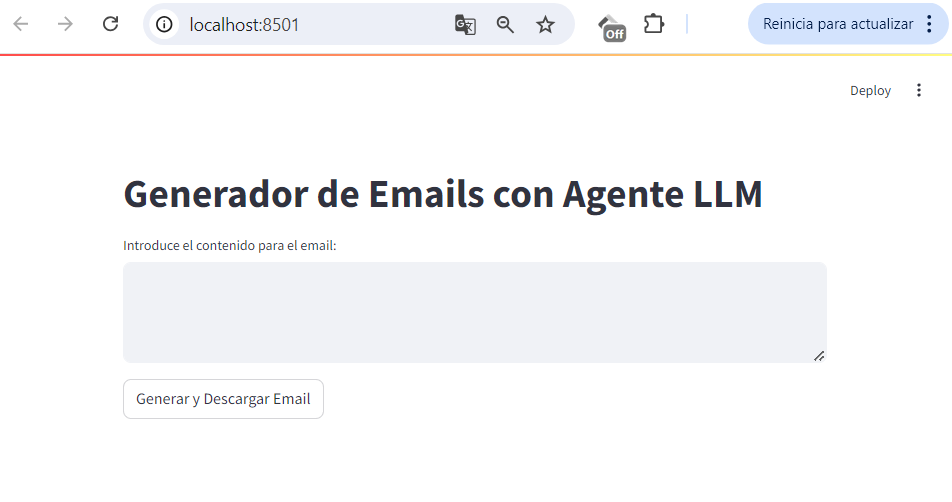
\includegraphics[width=1\linewidth]{Figures/interfaz_generador_email.png}
    \caption{Interfaz gráfica de la solución.}
    \label{fig:interfaz}
\end{figure}

La función principal en este proceso es la denominada \texttt{generar\_html\_y\_zip}. Dentro de esta se llama a la función \texttt{agent\_generate\_email} que es la que ejecuta el primer agente y desencadena todo el proceso hasta obtener el HTML final y las imágenes creadas. Posteriormente, utiliza la biblioteca zipfile para guardar el código HTML en un archivo \texttt{index.html} y para seleccionar las imágenes y encapsularlas en una carpeta \texttt{img}.

La funcionalidad de poder descargar un archivo ZIP es clave para este trabajo ya que es un requerimiento que el \textit{output} sea una carpeta que contenga la estructura de archivos necesaria para cargar el email en Adobe Campaign. Gracias a esta se logró un resultado acorde a lo que el cliente necesita.

%-------------------------------------------------------------------------------------------------------------
%-------------------------------------------------------------------------------------------------------------

\section{Integración de la solución}

En la figura~\ref{fig:diagrama_solucion} se puede observar un diagrama que resume todos los módulos que componen este trabajo y que hacen posible la generación de emails de forma automática. También se detalla el nombre del archivo .py donde se encuentra el código para cada parte.

\begin{figure}[!htpb]
    \centering
    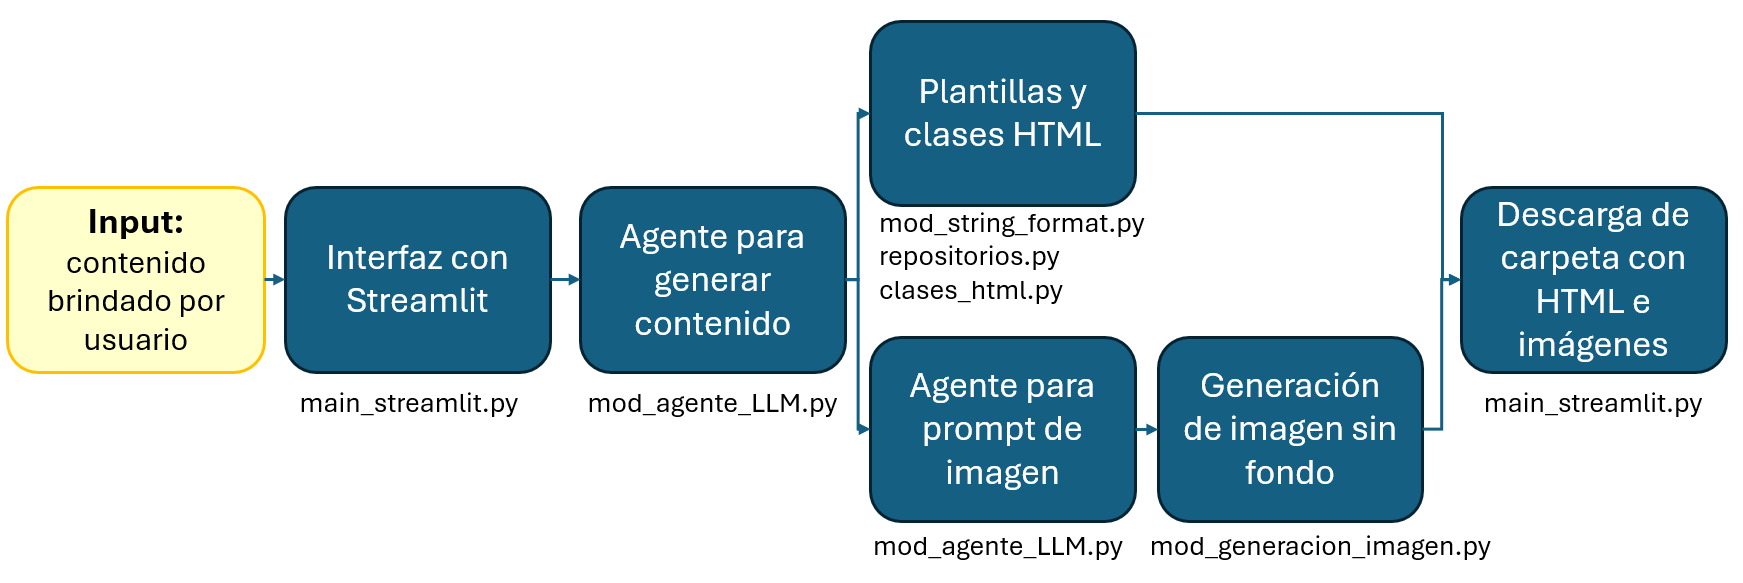
\includegraphics[width=\textwidth]{./Figures/diagrama_solucion_emails.png}
    \caption{Diagrama de la solución.}
    \label{fig:diagrama_solucion}
\end{figure}

Para recapitular lo explicado en las anteriores secciones, se puede resumir el proceso en las siguientes etapas:

\begin{itemize}
    \item El usuario utiliza la interfaz gráfica para enviar como \textit{input} el mensaje que quiere transmitir con el email, con todo el detalle que se quiere comunicar.
    \item Una vez que el usuario presiona el botón, se ejecuta una función que llama al primer agente LLM y le comparte el \textit{input}. 
    \item Este agente revisa el contenido y genera los elementos de texto del email (título, párrafo inicial, nombre de la imagen de cabecera, entre otros.). Posteriormente coloca estos componentes en \texttt{elementos\_str}, que es una variable de texto con formato JSON. Esta sirve de \textit{input} tanto para crear las clases HTML, como para generar la imagen de cabecera.
    \item La variable \texttt{elementos\_str} es decodificada y convertida en un diccionario de Python. Luego, cada elemento es asignado a la clase correspondiente. Finalmente todas las clases y elementos se utilizan para crear una instancia de la clase \texttt{Email\_HTML}. Se ejecuta el método \texttt{constructor\_html} de esta instancia para generar el HTML final.
    \item A su vez, la misma variable \texttt{elementos\_str} es enviada al siguiente agente LLM que analiza el contenido del email y crea un \textit{prompt} para generar la imagen de cabecera.
    \item Este \textit{prompt} se envía posteriormente a la función \texttt{generar\_imagen\_final} que engloba tanto la creación de la imagen en bruto, como la remoción del fondo.
    \item Finalmente, tanto el código HTML como las imágenes son guardados dentro de una carpeta comprimida que es descargada por el usuario.
\end{itemize}

Con este proceso se logra una integración fluida de todas las partes del sistema, lo que permite que los usuarios generen y descarguen emails personalizados y visualmente coherentes con facilidad.

% Chapter Template

\chapter{Ensayos y resultados} % Main chapter title

\label{Chapter4} % Change X to a consecutive number; for referencing this chapter elsewhere, use \ref{ChapterX}

En este capítulo se describen los ensayos que se realizaron y las métricas obtenidas. Además, se detallan los errores más comunes encontrados y ejemplos de estos casos.
%----------------------------------------------------------------------------------------
%	SECTION 1
%----------------------------------------------------------------------------------------

\section{Descripción de los ensayos realizados}
\label{sec:pruebasHW}

Con el fin de probar tanto el modelo de generación de texto, como la diferencia de resultados entre Stable Image Ultra y Stable Image Core, se prepararon diez \textit{prompts} diferentes con los cuales se generaron tres emails distintos para cada uno. El texto completo de estos \textit{prompts} se puede revisar en el apéndice~\ref{AppendixB}.

Para poder comparar correctamente los resultados de los dos modelos de generación de imagen, se le pidió al agente LLM que genere la descripción de la imagen y esta fue compartida a ambos modelos por igual. De esta forma se aísla la influencia del \textit{prompt} del resultado de la comparación.

Por otro lado, para los resultados del modelo de generación de texto, se separó el conteo del error en el formato JSON del resto de errores. Esto es debido a que el error con el \textit{parser} de JSON sucede al inicio y detiene todo el proceso, por lo que impide que se genere algún resultado que se pueda examinar más en profundidad. En los casos en los que surgía este error simplemente se volvía a ejecutar la función hasta que se genere un email. Igualmente se ha contabilizado el número de incidencias para analizarlo junto con los demás resultados.

En la tabla~\ref{tab:metricas_experimentos} se pueden observar los porcentajes de aceptación de cada modelo. Cabe resaltar que la aceptación se definió por juicio personal e implica que el resultado se puede utilizar en la práctica ya que no presenta errores mayores. Para los modelos de generación de imágenes se agregó una línea más para eliminar el efecto del error al remover el fondo, ya que este depende del modelo de edición más que del modelo de generación.

\begin{table}[ht]
	\centering
	\caption{Métricas de los ensayos.}
	\begin{tabular}{l c c c}    
		\toprule
		\textbf{Métrica} & \textbf{Texto} & \textbf{S. I. Ultra} & \textbf{S. I. Core} \\
		\midrule
		\% de aceptación & 73,3\% & 40,0\% & 43,3\% \\
            \% de aceptación sin error de fondo & - & 73,3\% & 56,7\% \\
		\bottomrule
		\hline
	\end{tabular}
	\label{tab:metricas_experimentos}
\end{table}

En la tabla~\ref{tabla:resultados_experimentos} se puede revisar el detalle de todas las pruebas realizadas con las observaciones encontradas tanto del modelo de texto y como de los dos modelos de generación de imágenes. También se puede ver el conteo de errores en el formato JSON, que representa el 30\% de las ejecuciones totales.

Como se puede observar, aún existe camino por recorrer para mejorar la efectividad de todos los modelos, con especial énfasis en los de generación de imágenes y edición. En las próximas secciones se describe en detalle los errores más comunes observados.

\begin{table}[ht]
\centering
\scriptsize % Cambia el tamaño de la letra a pequeño
\caption{Detalle de ensayos y resultados.} 
\label{tabla:resultados_experimentos}
\begin{tabular}{c c l l l}
\toprule
\textbf{Prueba} & \textbf{\# Error JSON} & \textbf{Texto} & \textbf{Imagen S. I. Ultra} & \textbf{Imagen S. I. Core} \\
\midrule
1.1 & 2 & Ok & Error mano y objeto. & Ok \\
1.2 & 0 & Error legal. & Error mano. & Ok \\
1.3 & 0 & Ok & Error mano y fondo. & Error brazo. \\
2.1 & 0 & Ok & Ok & Error mano. Error caras. \\
2.2 & 2 & Ok & Ok & Error fondo. Error ojos. \\
2.3 & 0 & Ok & Error fondo. & Error fondo. \\
3.1 & 0 & Falta signo ``!''. & Ok & Error mano e interpretación. \\
3.2 & 3 & Ok & Error mano. & Error brazo. \\
3.3 & 2 & Ok & Ok & Error mano. \\
4.1 & 0 & Error espacios. & Error fondo. & Ok \\
4.2 & 0 & Ok & Error fondo. & Ok \\
4.3 & 0 & Ok & Ok & Error mano. Error fondo. \\
5.1 & 0 & Ok & Ok & Ok \\
5.2 & 0 & Ok & Ok & Error fondo. Chica con bigote. \\
5.3 & 1 & Ok & Error mano. & Ok \\
6.1 & 0 & Ok & Error fondo. & Ok \\
6.2 & 0 & Ok & Error fondo. & Ok. Mejorar temática. \\
6.3 & 0 & Ícono no existe. & Error mano y fondo. & Ok. Mejorar temática. \\
7.1 & 1 & Ok & Ok & Ok \\
7.2 & 0 & Error texto de íconos. & Error mano y fondo. & Error fondo. \\
7.3 & 0 & Ok & Error fondo. & Error mano. \\
8.1 & 0 & Ícono no existe. & Error mano y fondo. & Ok \\
8.2 & 0 & Ícono no existe. & Error fondo. & Ok \\
8.3 & 0 & Error ícono y legal. & Ok & Error fondo. \\
9.1 & 0 & Ok & Ok & Chica con bigote. \\
9.2 & 0 & Ok & Error fondo. & Error ojos. \\
9.3 & 0 & Ok & Ok & Error mano. \\
10.1 & 0 & Ok & Error fondo. & Error mano. \\
10.2 & 2 & Ok & Error piernas. & Fuera de tema. \\
10.3 & 0 & Ok & Ok & Ok \\
\bottomrule
\hline
\end{tabular}
\end{table}


A pesar de los errores, es importante notar lo fácil, rápido y económico que resultó crear diez emails con tres versiones distintas de cada uno. Si bien cada prueba individual puede presentar errores, la variedad de versiones que se generan hace posible que exista por lo menos una opción adecuada para casi todos los \textit{prompts}. 

Por ejemplo, para el \textit{prompt} número uno, si se escoge el email generado en la prueba uno con la imagen de Stable Image Core se obtiene el excelente resultado de la figura~\ref{fig:prueba_1_1}. Lo mismo ocurre con el \textit{prompt} cuatro, prueba dos, imagen del servicio Core, que se puede observar en la figura~\ref{fig:prueba_4_2}. Adicionalmente, se muestra en la figura~\ref{fig:prueba_9_1} el resultado del \textit{prompt} nueve, prueba uno y la imagen de Stable Image Ultra. 

Estos tres ejemplos son una muestra pequeña de la variedad de emails que pueden ser generados en cuestión de minutos.

\begin{figure}[H]
    \centering
    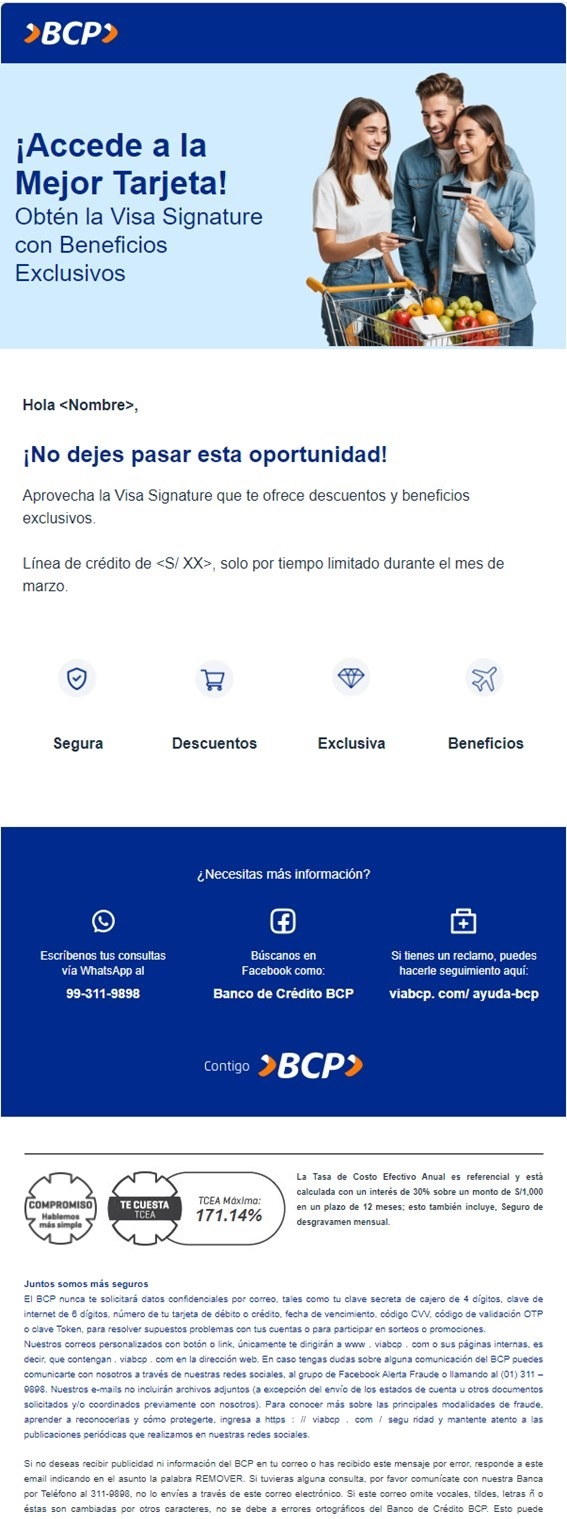
\includegraphics[width=0.6\linewidth]{Figures/Prueba_1_1_core.JPG}
    \caption{Resultado del \textit{prompt} uno, prueba uno y S. I. Core.}
    \label{fig:prueba_1_1}
\end{figure}

\begin{figure}[H]
    \centering
    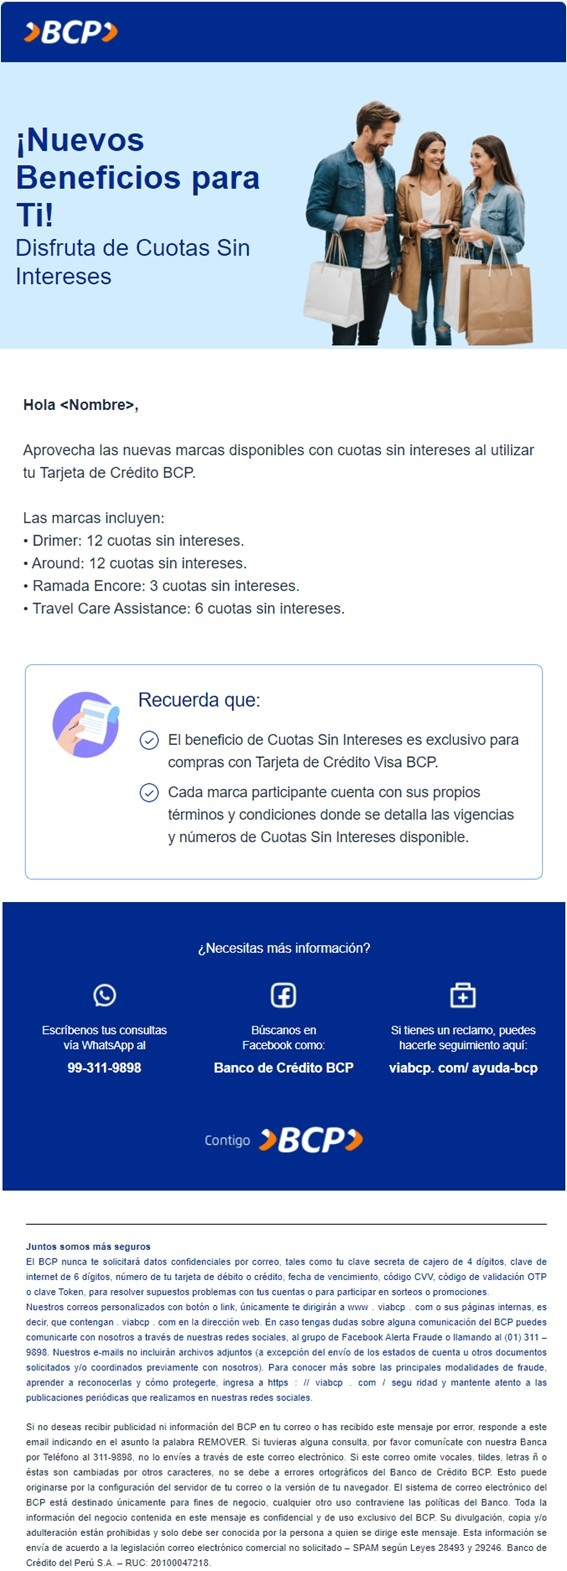
\includegraphics[width=0.6\linewidth]{Figures/Prueba_4_2_core.JPG}
    \caption{Resultado del \textit{prompt} cuatro, prueba dos y S. I. Core.}
    \label{fig:prueba_4_2}
\end{figure}

\begin{figure}[H]
    \centering
    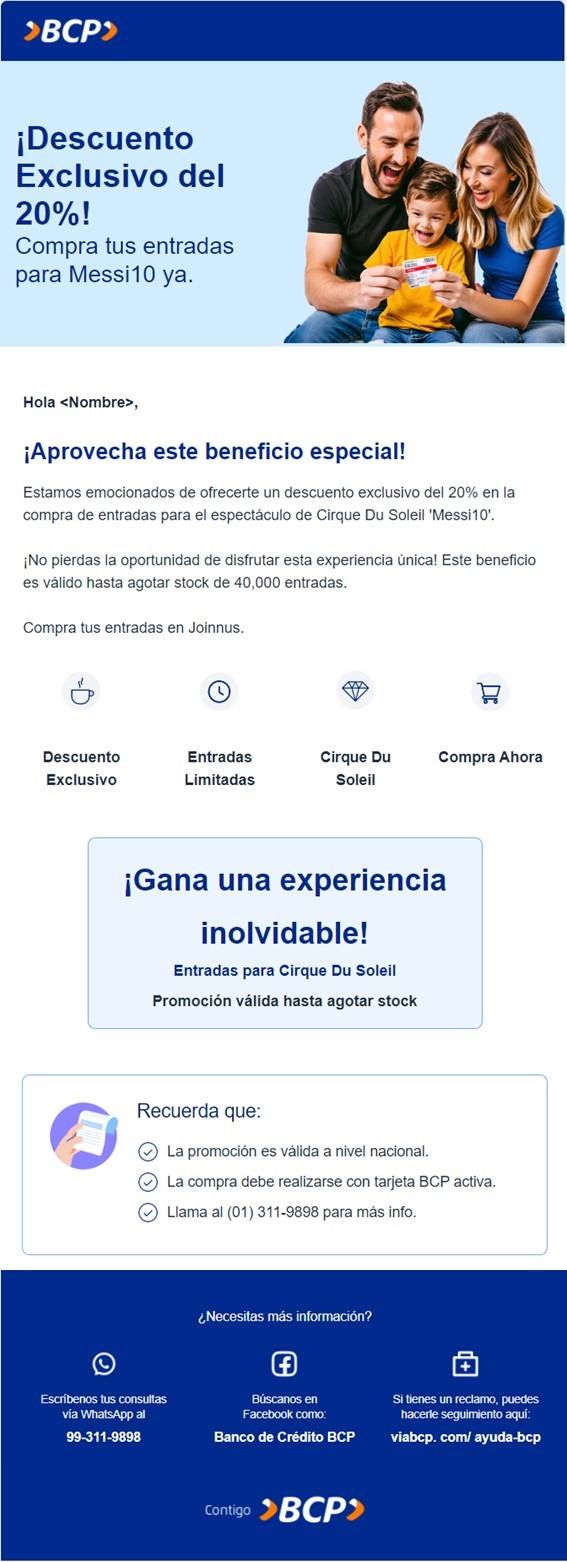
\includegraphics[width=0.6\linewidth]{Figures/Prueba_9_1_ultra.JPG}
    \caption{Resultado del \textit{prompt} nueve, prueba uno y S. I. Ultra.}
    \label{fig:prueba_9_1}
\end{figure}

\section{Errores más comunes del modelo de texto}

Como se mostró en la sección anterior, el modelo de texto en general obtiene excelentes resultados con un porcentaje de aceptación de 73,3\%. Uno de los errores más comunes es la dificultad para agregar correctamente la sección legal de la tasa. Esto se puede deber en parte a que es mucho texto que se tendría que identificar y copiar intacto. Una posible solución es modificar la interfaz para compartir el texto legal deseado en un recuadro aparte. Este contenido no se enviaría al LLM sino que se insertaría directamente en la plantilla. Con este enfoque, aparte de solucionar los errores, se volvería más eficiente la inclusión del legal.

Otro error visto es omitir revisar la lista de íconos disponibles e inventar los nombres de estas imágenes. También, en una ocasión el texto que acompañaba a los íconos resultó incoherente. Un plan de acción para mitigar estos problemas sería crear un agente especializado en configurar este tipo de secciones, que requieren un poco más de atención en los detalles.

El resto de errores, como la falta de un signo de exclamación inicial o la necesidad de agregar más espacios, son menos comunes. En general, el modelo capta bastante bien lo que hay que comunicar y lo realiza de una forma profesional acorde a lo que el cliente necesita.

Un aspecto que sí es importante considerar son los errores al brindar un formato JSON. Estas incidencias se dieron un tercio de las veces que se ejecutaba la función, por lo que son bastante frecuentes. El problema más común observado es que el LLM coloca la palabra ``JSON`` de esta manera: \texttt{ json \{ item: contenido, item: contenido\}}. Una solución fácil de implementar que disminuiría estos errores sería buscar y reemplazar la palabra ``JSON`` antes de enviar el contenido al parser. También se puede crear un agente validador, cuya tarea sea únicamente corregir cualquier error en el formato.

\section{Errores más comunes de los modelos de generación de imágenes y comparación}

Por el lado de la generación de imágenes se identificaron más aspectos para mejorar. Un error común, no solo de los modelos de Stability AI sino de los modelos de generación de imágenes en general, se presenta al graficar manos y extremidades. Se han encontrado errores diversos en esta área, como dedos adicionales, manos flotantes sosteniendo bolsas de compra, brazos más largos de lo normal, o falta de una pierna. En la figura ~\ref{fig:erroresManos} se muestran ejemplos de estos casos.

\begin{figure}[H]
    \centering
    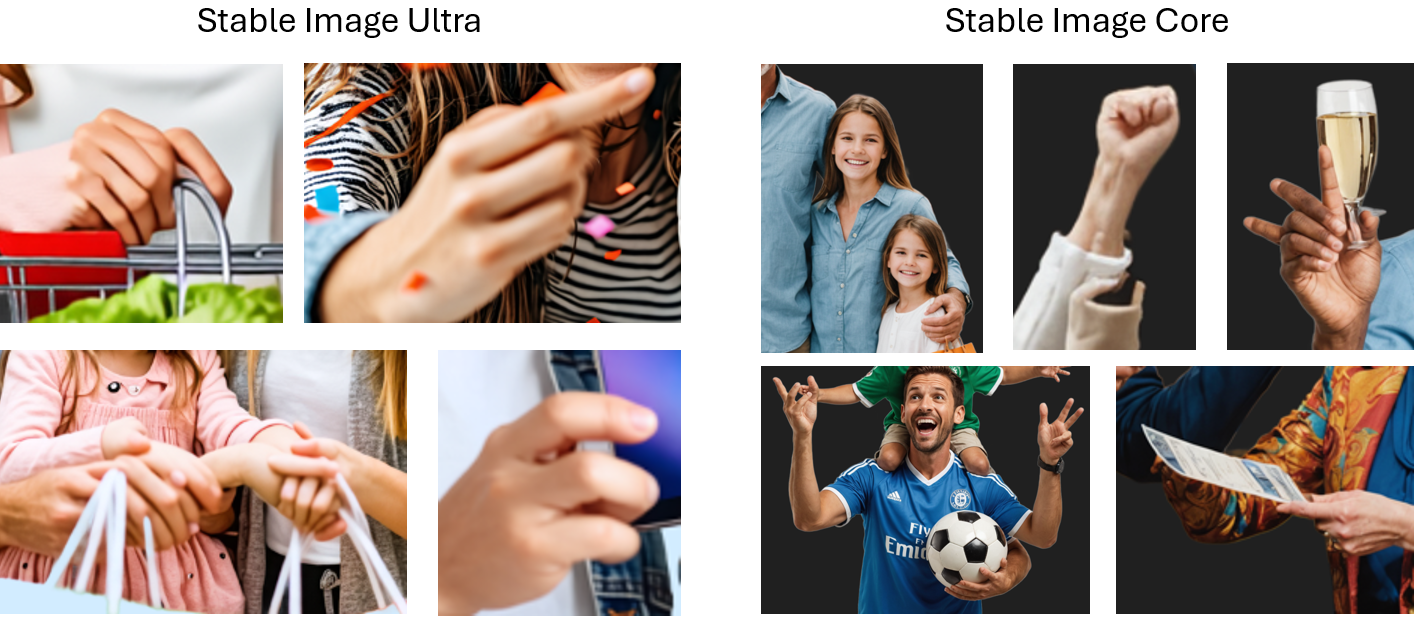
\includegraphics[width=1\linewidth]{Figures/erroresManos.png}
    \caption{Ejemplos de errores al graficar manos.}
    \label{fig:erroresManos}
\end{figure}

Otro tipo de error que se ha observado sobre todo en Stable Image Core es el de crear rostros distorsionados, con los ojos sin definir o viendo en dos direcciones diferentes. Además, este modelo tiende a colocar bigotes incluso en mujeres. Este tipo de errores se disminuyen al utilizar Stable Image Ultra. En la figura~\ref{fig:erroresManos} se pueden ver algunos ejemplos.

\begin{figure}[H]
    \centering
    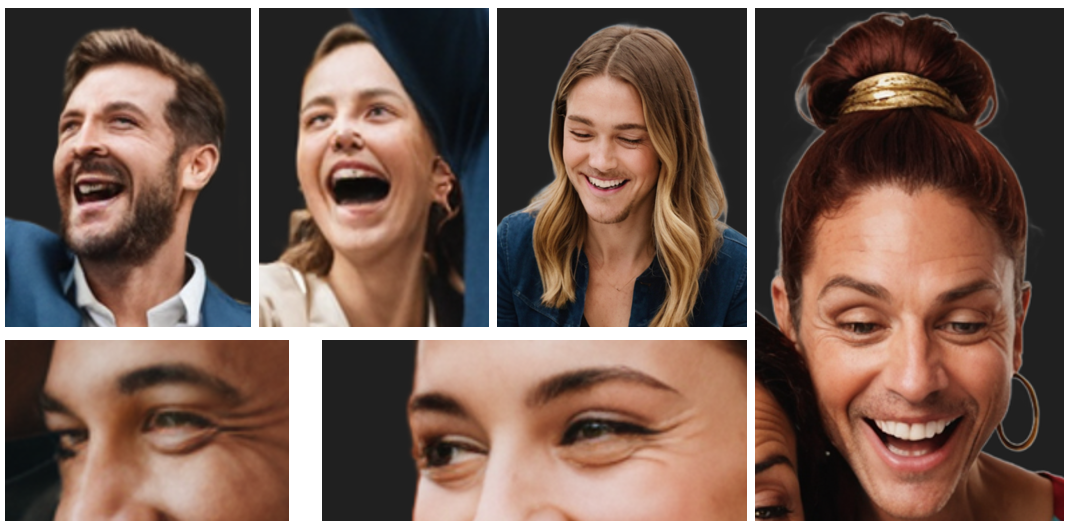
\includegraphics[width=1\linewidth]{Figures/erroresRostros.png}
    \caption{Ejemplos de errores al graficar rostros.}
    \label{fig:erroresManos}
\end{figure}

Por último, existen ocasiones en que, al remover el fondo, se quitan elementos que no correspondía eliminar. Esto ha pasado con mayor frecuencia al utilizar el servicio Stable Image Ultra, pero es un error que corresponde más a la herramienta de edición de imágenes. En la figura~\ref{fig:erroresFondo} se muestran ejemplos de este error.

\begin{figure}[H]
    \centering
    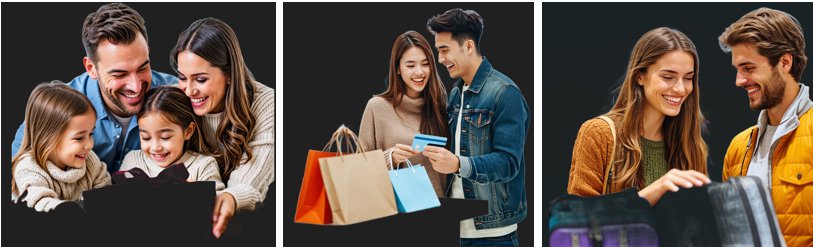
\includegraphics[width=1\linewidth]{Figures/erroresFondo.png}
    \caption{Ejemplos de errores de remoción de fondo.}
    \label{fig:erroresFondo}
\end{figure}

Una alternativa es evitar este paso al colocar la imagen completa como fondo de cabecera. Para lograrlo, se tendrían que realizar algunos pasos adicionales luego de generar la imagen. El primero sería hacer un escalado de la imagen para volverla más ancha de un lado. Luego se tendría que recortar para lograr el tamaño exacto de la cabecera. Finalmente, se debería imprimir el título del email sobre la imagen. 

Para clarificar, se puede observar un ejemplo en la figura~\ref{fig:cabeceraAlternativa}. Este tipo de diseño de cabecera ya es utilizado por la empresa y sería una alternativa interesante que quedaría pendiente por explorar.

\begin{figure}[H]
    \centering
    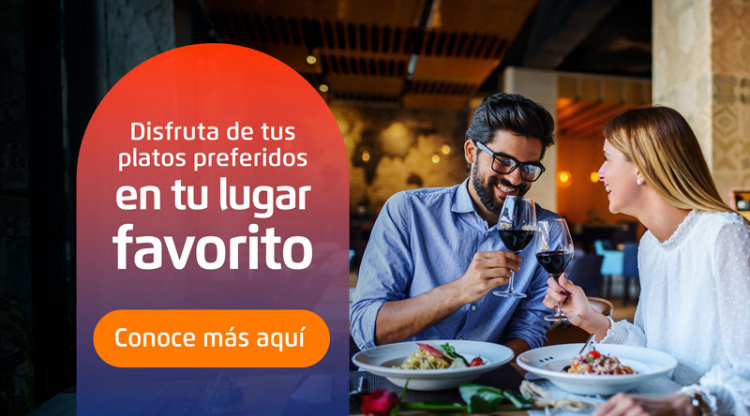
\includegraphics[width=0.8\linewidth]{Figures/cabeceraAlternativa.png}
    \caption{Ejemplo de cabecera con imagen de fondo y título impreso encima.}
    \label{fig:cabeceraAlternativa}
\end{figure}

Luego de analizar los resultados queda pendiente resolver qué servicio es mejor utilizar, si Stable Image Core o su versión Ultra. Es difícil afirmar que el mayor precio del Ultra se compensa con sus mejores resultados ya que, como se mencionó anteriormente, su precio es 2,6 veces superior al servicio Core pero su aumento de efectividad no es el doble. Es cierto que al omitir el paso de la remoción del fondo, este modelo obtiene mejores resultados. Sin embargo, se puede concluir que conviene seguir generando alternativas de imágenes con ambos modelos para tener mayor variedad entre las cuales elegir.
 
% Chapter Template

\chapter{Conclusiones} % Main chapter title

\label{Chapter5} % Change X to a consecutive number; for referencing this chapter elsewhere, use \ref{ChapterX}


%----------------------------------------------------------------------------------------

%----------------------------------------------------------------------------------------
%	SECTION 1
%----------------------------------------------------------------------------------------
En este capítulo se resaltan las conclusiones más importantes y las recomendaciones a seguir para mejorar la solución planteada en este trabajo.

\section{Conclusiones generales }

Luego de haber revisado el desarrollo de este trabajo, se pueden realizar las siguientes conclusiones:

\begin{itemize}
\item En general, se lograron cumplir todos los requerimientos planteados en la planificación del proyecto. Se pudo crear una solución que genera emails en cuestión de minutos en el formato que el cliente solicitó, con una interfaz gráfica fácil de usar, incluso sin conocimiento técnico. En el aspecto de seguridad, si bien se está usando APIs de terceros, esta es una alternativa aceptada por el cliente.
\item Ya que la inteligencia generativa está en un momento de constantes cambios, este trabajo se vio beneficiado por tener a disposición modelos fundacionales de muy buena calidad. Si bien esto exigió cambios en la planificación original y actualizaciones del desarrollo a mitad de camino, fue a favor del resultado final.
\item Se manifestó el riesgo relacionado a no poder obtener ayuda de la empresa para recopilar grandes cantidades de emails. Sin embargo, finalmente se pudieron conseguir algunos ejemplos que bastaron para el desarrollo del trabajo ya que no fue necesario entrenar un modelo desde cero o realizar \textit{fine tuning}.
\end{itemize}

%----------------------------------------------------------------------------------------
%	SECTION 2
%----------------------------------------------------------------------------------------
\section{Próximos pasos}

Existen varias formas en las que se puede seguir mejorando este trabajo. A continuación se describen algunas de ellas.

\begin{itemize}
    \item Interfaz gráfica: para tener un producto más robusto, queda pendiente construir una página web con algún framework de desarrollo web como React o Angular. Adicionalmente, dentro de la interfaz se pueden incluir las siguientes funcionalidades:
    \begin{itemize}
        \item Tener un usuario donde se puedan almacenar los emails creados anteriormente.
        \item Poder iterar sobre un email creado y modificarlo.
        \item Tener campos para ingresar los textos legales.
        \item Poder visualizar y seleccionar entre diferentes versiones de email o de imágenes de cabecera.
        \item Crear varias versiones del email para cada segmento de clientes en una sola solicitud.
    \end{itemize}
    \item Generación de texto y HTML:
    \begin{itemize}
        \item Crear más clases de elementos opcionales. Por ejemplo: sección para incluir GIFs, botón de link, lista de descuentos, entre otras.
        \item Incorporar las plantillas para otros segmentos de clientes como Enalta y Privada.
        \item Probar una clase opcional libre en la que se deje a un agente LLM crear una parte del código HTML desde cero.
        \item Utilizar RAG (\textit{retrieval augmented generation} por su sigla en inglés) \cite{NEURIPS2020_6b493230} o \textit{fine tuning} para enseñarle al modelo terminología bancaria propia de la empresa y conocimiento general sobre los productos y servicios que brinda.
        \item Mantener actualizada la solución con los últimos modelos, ya sea de OpenAI, Google, Anthropic, Meta, u otro.
        \item Implementar un modelo LLM en entorno privado para asegurar una máxima confidencialidad de la información.
    \end{itemize}
    \item Generación de imágenes: este constituye el aspecto que más errores puede ocasionar. Debido a esto, se sugieren varias formas de prevenirlos:
    \begin{itemize}
        \item Utilizar modelos de edición de imágenes para poder corregir detalles como manos mal dibujadas u objetos flotantes.
        \item Generar varias imágenes y seleccionar las opciones más apropiadas con el uso de modelos de visión por computadora como GPT-4V \cite{openai2023gpt4v} o las versiones Omni de GPT.
        \item Eliminar el paso de remoción de fondo usando la imagen completa como fondo e imprimiéndole encima el título del email.
        \item Seguir experimentando con repositorios de contenido multimedia para algunos casos de uso. Por ejemplo, se puede tener un repositorio de GIFs para poder incorporar al email.
        \item Mantener actualizada la aplicación con los últimos modelos para que los resultados se perfeccionen con el tiempo.
    \end{itemize}
\end{itemize}

Existen muchas posibilidades para optimizar la solución planteada. Sin lugar a dudas la inteligencia artificial generativa tiene el potencial de agilizar no solo este proceso de creación de emails, sino que se puede extender a varios casos de uso de desarrollo de contenido. Experimentar y combinar diferentes técnicas, herramientas y modelos es lo que permitirá encontrar soluciones óptimas a problemas de automatización como este y sacarle el máximo provecho a estas tecnologías. 

%----------------------------------------------------------------------------------------
%	CONTENIDO DE LA MEMORIA  - APÉNDICES
%----------------------------------------------------------------------------------------

\appendix % indicativo para indicarle a LaTeX los siguientes "capítulos" son apéndices

% Incluir los apéndices de la memoria como archivos separadas desde la carpeta Appendices
% Descomentar las líneas a medida que se escriben los apéndices

%% Appendix A

\chapter{\textit{Prompt} de la herramienta \texttt{create\_email}} % Main appendix title

\label{AppendixA} % Change X to a consecutive letter; for referencing this appendix elsewhere, use \ref{AppendixX}

En este apéndice se puede observar el \textit{prompt} completo que le explica al agente de inteligencia artificial cómo usar la función \texttt{create\_email}.

\section{\textit{Prompt} }

`` Útil para crear el código html de un email en base al contenido que se le de en los inputs.

    Inputs para la función create\_email: brindar un str con formato json que contenga estos elementos obligatorios (no incluir la palabra json en el input):
        \begin{quote} 
        segmento\_cliente: str, nombre\_imagen\_cabecera: str,titulo1: str,titulo2: str, parrafo\_inicial:str
        \end{quote}
        
    También se puede optar por incluir elementos opcionales de esta lista:
        \begin{quote} 
        frase\_inicial:str, tcea\_trea:str, tasa:str, texto1\_tasa:str, texto2\_tasa:str , texto\_iconos:List[str], iconos:List[str], recuadro\_premio:List[str], recuadro\_lista:List[str], orden:List[str]
        \end{quote}
    A continuación la descripcion de los valores que deben ir en el contenido de los elementos:
        \begin{quote} 
        segmento\_cliente: Segmento de cliente al que va dirigido el email. Puede ser ``Bex'' o ``Consumo''.
        
        nombre\_imagen\_cabecera: Nombre de la imagen que se usará dentro de la cabecera y que se insertará en el código html. Debe contener la extensión .png.
        
        titulo1: Primera parte del título que irá en la cabecera. Es la primera línea que irá resaltada en negrito, debe tener la frase más importante.
        
        titulo2: Segunda parte del título que irá en la cabecera. Puede ser la continuación del titulo1, o una oración aparte. Debe ser una frase breve que no necesite comas.
        
        parrafo\_inicial: Es el primer párrafo en el cuerpo del email, debe contener la información más relevante que se quiere comunicar al cliente. Puedes agregar <br><br> entre lineas para dividir el párrafo si lo ves apropiado.


        frase\_inicial: Una frase que irá antes del párrafo inicial. Es una sola oración de preferencia con signos de exclamación y va resaltada en azúl en el email. Que sea diferente al título y al párrafo inicial para que no suene redundante.
        
        tcea\_trea: En caso se especifique alguna tasa de interés que se deba incluir en el email, en este campo se debe especificar qué tipo de tasa es: ``TREA'' o ``TCEA''. Si no te brindan el valor de la tasa, no enviar este campo.
        
        tasa: colocar el valor de la TREA o TCEA brindada. Puede ser un valor o un rango. Ej1: "120%". Ej2:"5%-8%" Si no te brindan el valor de la tasa, no enviar este campo.
        
        texto1\_tasa: Incluir el descriptivo de la tasa enviada, tal cual te la dan sin ningún cambio. En caso se tenga TREA, enviar el descriptivo de la tasa mínima. En caso se tenga TCEA, enviar todo el descriptivo. Si no te brindan el valor de la tasa, no enviar este campo.
        
        texto2\_tasa: Solo usar en caso se tenga TREA. Enviar el descriptivo de la tasa máxima, tal cual te la dan sin ningún cambio. Si no te brindan el valor de la tasa, o si la tasa es TCEA, no usar este campo.
        
        texto\_iconos: lista de 4 características cortas que tiene el producto, servicio o promoción que se está comunicando y que se buscan mencionar al cliente. Deben ser hasta 3 palabras máximo cada texto y la primera palabra debe empezar con mayúscula.
        
        iconos: lista de los nombres de las imágenes de 4 iconos que acompañarán a cada elemento de la lista texto\_iconos. Se deben seleccionar de estas opciones de iconos: \{iconos\_img\}
        
        recuadro\_premio: lista de 3 líneas de texto. Sirve para resaltar un solo premio o beneficio que el cliente puede ganar. Este premio es descrito en 3 lineas de texto. La primera línea es la que se muestra más grande, y las otras 2 menos resaltadas. Ejemplo: [``¡Gana una Auto!",``Kia Sorrento 0 Km'',``Sorteo:15 de setiembre'']
        
        recuadro\_lista: sirve para enlistar una serie de instrucciones, pasos o recordatorios al cliente. El número de elementos es variable, pero el primer elemento siempre es el título de la lista. Este primer elemento puede ser ``Ten en cuenta:'', ``Recuerda que:'',``Sigue estos pasos:'' o algo similar. El resto de elementos son los textos a enlistar.
        
        orden: En caso se utilicen más de uno de estos elementos (iconos, recuadro\_premio, recuadro\_lista ), enviar el orden en el que deben aparecer. Ejemplo: orden= [``iconos'', ``recuadro\_premios", \\``recuadro\_lista'']
        \end{quote}
    Si te piden colocar algún dato como campo personalizado, envíalo en el contenido del elemento que corresponda con el dato entre estos símbolos:``\&lt; dato \&gt;''. No utilices los simbolos ``<>'' para este propósito.
    
    No menciones clientes Bex o Consumo en el contenido del mail, son palabras de uso interno.
    
    El input debe ser en formato json con los elementos elegidos debidamente separados con coma. Si olvidas alguna coma, se generará un error. No olvidar comas.
    ''
%% Appendix A

\chapter{\textit{Prompts} de los ensayos} % Main appendix title

\label{AppendixB} % For referencing this appendix elsewhere, use \ref{AppendixA}

En este apéndice se detallan los \textit{prompts} de usuario que se han probado para generar emails de diversas temáticas.

\section{\textit{Prompt} 1}

``Crea un email para vender tarjetas de crédito a clientes Consumo. Resalta a los clientes que tienen acceso a la mejor tarjeta, Visa Signature, que les brinda descuentos y beneficios exclusivos, con una línea de crédito de <S/ XX>, solo por tiempo limitado durante el mes de marzo. 

Incluir el monto de la línea de crédito que está entre <> como campo personalizado.

Menciona estos 4 beneficios de la tarjeta: es segura, descuentos en compras, es exclusiva, beneficios al viajar
TCEA: 171.14\%

Legal de la TCEA: La Tasa de Costo Efectivo Anual es referencial y está calculada con un interés de 30\% sobre un monto de S/1,000 en un plazo de 12 meses; esto también incluye, Seguro de desgravamen mensual. Si te retrasas en el pago se te cobrará una tasa de interés moratorio de 12.51\% en soles y 10.26\% en dólares.''


\section{\textit{Prompt} 2}


``Phillip Chu Joy y El cuy mágico se juntaron para hacer el evento más regalón del
año con “el regalaton del cuy mágico” donde premiarán a los ahorradores de las
cuentas BCP. Serán 10 ganadores y pueden llevarse premios hasta de 200mil soles
cada uno.
Para participar, debes incrementar 100 soles en CUALQUIER cuenta de ahorros
desde el 1 de noviembre al 15 de diciembre.

Además, podrás participar de sorteos semanales en la web en la ruleta.
PARTICIPAN TODAS LAS CUENTAS
Premios:

Premio Regalatón:
Auto Jeep Renegade 2023 Sport,
Giftcard Vale Consumo,
Paquete doble de crucero,
Pack deportivo selección(Camiseta y buzo),

Play Station 5,
Nintendo Swtich,
Home Theater,
Macbook Pro 13 M2 256GB,
Iphone 15 128 GB,
Ipad Pro 11 M2 128GB,
Smart TV 70 \&\#39; Samsung,
Scooter Eléctrico Xiaomi 4 Pro,
Tomatodo,
Dinero en efectivo.

Premios Semanales:
Premio
Cashback S/10,
Cashback S/20,
Cashback S/50,
Camisetas Selección,
Twelve Pack Pilsen TADA,
Vale restaurante/supermercado,
Giftcard varios''


\section{\textit{Prompt} 3}

``Crea un email para invitar a los clientes a participar en la promoción 'Jugada del Cuy', donde pueden ganar hasta S/20,000.  Incluye un título atractivo que anime a los clientes a entrar en modo fútbol y ahorrar. Detalla los pasos para participar: 'Entrar al campo' registrándose, 'Golear con los depósitos' acumulando puntos por cada S/100 incrementado en sus cuentas, y 'Multiplicar y anotar' acertando el marcador para duplicar los puntos. Asegúrate de incluir íconos para cada paso.

TREA: 0.00\%
Legal tasa: TREA referencial de 0\% para la Cuenta Digital BCP considerando un monto de S/1,000 a 12 meses. Interés acumulado: S/ 0.00. Depósitos cubiertos por el Fondo de Seguros de Depósitos que varía trimestralmente. Para conocer monto actualizado, visite www. fsd. org. pe. Tarifario y condiciones llamando al (01) 311-9898 o ingresando a www. viabcp. com.''

\section{\textit{Prompt} 4}

``Crea un email para promocionar los nuevos beneficios de las tarjetas de crédito BCP. explica que ahora se pueden aprovechar nuevas marcas con cuotas sin intereses: Drimer (marca de colchones) - 12 cuotas sin intereses; Around (marca de maletas) - 12 cuotas sin intereses; Ramada Encore (marca de hoteles) - 3 cuotas sin intereses.; Travel Care Assitance (marca de seguros para viajes) - 6 cuotas sin intereses.

Al final, incluye un recordatorio sobre las condiciones del beneficio de cuotas sin intereses:
- El beneficio de Cuotas Sin Intereses es exclusivo para compras con Tarjeta de Crédito Visa BCP.
- Cada marca participante cuenta con sus propios términos y condiciones donde se detalla las vigencias y números de Cuotas Sin Intereses disponible.''

\section{\textit{Prompt} 5}

``Crea un email para anunciar la preventa exclusiva de los nuevos dispositivos Galaxy Z. Resalta que los clientes pueden acumular millas adicionales al comprar en cuotas sin intereses usando su tarjeta de crédito Visa LATAM Pass. Incluye imágenes de los dispositivos Galaxy Z con los bonos de millas que se pueden ganar y un botón para conocer más detalles. Agrega una sección al final que recuerde que este beneficio es exclusivo para compras en canales online.

TCEA: 171.14%

T\&C: Promoción a nivel nacional vigente del 26 de agosto al 15 de setiembre del 2024. Esta campaña es desarrollada por el Banco de Crédito del Perú (BCP). Premio: por la compra de un equipo Z Fold 6 512GB obtén un bono de extra millas de 2,000 millas LATAM Pass y por la compra de un equipo Z Flip 6 512GB obtén un bono de extra millas de 1,000 millas LATAM Pass. Solo se aplicará un premio por cliente. Participan clientes que compran un equipo Samsung Z Fold 6 (512GB o 1TB) o Z Flip 6 (512GB) en Cuotas Sin Intereses. Promoción válida hasta agotar stock. Stock de premios: 500 (Quinientos clientes). Un solo cliente podrá acumular un máximo de 2,000 millas utilizando el multiplicador mencionado. Participan los clientes titulares de Tarjetas de Crédito Visa BCP LATAM Pass que consuman los productos especificados de la promoción en cuotas sin intereses en el canal online de Samsung durante el periodo de vigencia de la promoción. Para más información sobre comercios participantes ingresa a https://www.viabcp.com/beneficios/cuotas-sin-intereses/samsung. Se consideran los consumos que el cliente realice con las Tarjetas de Crédito Visa BCP LATAM Pass que posea, incluyendo sus adicionales, siendo que, para este caso, las millas serán abonadas a favor del titular principal de la tarjeta. Se consideran únicamente los consumos realizados durante la vigencia de promoción y para los productos seleccionados para la promoción. Para efectos de entrega del Premio, es decir, las millas multiplicadas se realizarán los abonos en la cuenta de socio LATAMPASS a más tardar el 21/10/24 y corresponderá a las millas adicionales entregadas con ocasión de esta promoción. Para fines de abono la tarjeta de crédito del cliente debe encontrarse activa y sin bloqueo a la fecha de abono del premio, caso contrario el cliente perderá el derecho a recibir el premio. Para más información sobre la presente promoción, restricciones, costos y tributos aplicables a las Tarjetas de Crédito Visa BCP LATAM Pass llamar a nuestra Banca por Teléfono al 311-9898 o ingresar a viabcp.com.
''

\section{\textit{Prompt} 6}

``Crea un email para promocionar la campaña de canje de millas LATAM Pass. Ofrece un descuento de hasta el 60\% en el canje de millas pagando con tarjetas BCP. Debajo, agrega íconos que representen las opciones de canje: pasajes, hospedaje, productos del catálogo y gift cards.

TCEA:180.53\%

Legal tasa: La Tasa de Costo Efectivo Anual es referencial y está calculada con un interés de 30\% sobre un monto de S/1,000 en un plazo de 12 meses; esto también incluye, Seguro de desgravamen mensual. Si te retrasas en el pago se te cobrará una tasa de interés moratorio de 12.51\% en soles y 10.26\% en dólares.''

\section{\textit{Prompt} 7}

``Crea un email para invitar a los clientes a participar en un sorteo para ganar paquetes dobles al Caribe. Explica que los clientes pueden ganar participando por cada S/100 que incrementen en sus cuentas de ahorros BCP. Incluye un botón para registrarse en la promoción y destaca que la fecha límite para participar es el 29 de septiembre.

TREA:-14.40\%

Legal tasa:TREA Referencial para Cuenta llimitada BCP considerando un monto de S/1,000 a 12 meses y mantenimiento mensual de S/12. Interés acumulado: S/-144.00. Mayor información sobre condiciones, restricciones, costos, otros tipos de cuentas de ahorros, productos y disponibilidad de plataformas digitales ingresando a la página web www.viabcp.com.Depósitos cubiertos por el Fondo Seguro de Depósitos (FSD) que varia trimestralmente. Para conocer el monto actualizado visita www.fsd.org.pe. Mayor información de condiciones, restricciones, cargos y productos, llamar al 311 9898 o ingresa a productos, llamar al 311 9898 o ingresa a viabcp.com.

Términos y condiciones: “Paquetes al Caribe” Promoción válida a nivel nacional, vigente del 26 de julio al 29 de setiembre de 2024. Esta Promoción es desarrollada por el Banco de Crédito del Perú (BCP). Participan todas las personas naturales que durante la vigencia de la Promoción: (i) tengan o abran una Cuenta de Ahorros BCP, ya sea Digital, Premio, Ilimitada, Cuenta Sueldo y/o una o varias cuentas en la alcancía digital “Warda” del BCP (en adelante, las “Cuentas Participantes”); (ii) se inscriban en el siguiente formulario https://www.viabcp.com/promos-ahorros-bcp; y (iii) cumplan con los siguientes requisitos: (i) Clientes con Cuentas Participantes activas: Incrementar el saldo total, entre todas sus Cuentas Participantes, desde la fecha de inicio de la Promoción hasta un día antes de la fecha del sorteo, en un monto mínimo de S/100.00 (Cien y 00/100 Soles) o USD \$30.00 (Treinta y 00/100 Dólares Americanos). (ii) Personas que abrirán una nueva Cuenta Participante: Abrir una Cuenta Participante y mantenerla, hasta un día antes de la fecha del sorteo, con un saldo igual o mayor a S/100.00 (Cien y 00/100 Soles) o USD \$30.00 (Treinta y 00/100 Dólares Americanos) entre todas sus cuentas. En adelante, los “Clientes”. Si los Clientes cumplen con lo señalado acumularán una (1) opción para el sorteo. 

\section{\textit{Prompt} 8}

``Crea un email para invitar a los clientes a participar en una tómbola con premios como televisores, tablets, y más. Detalla los pasos para participar en la tómbola: acumular un monto mínimo de S/500 en compras, acercarse a la tómbola con el voucher, y ganar premios. Usa íconos para representar los premios disponibles y un botón para conocer más detalles.

TCEA:180.53\%

Legal tasa: La Tasa de Costo Efectivo Anual es referencial y está calculada con un interés de 30\% sobre un monto de S/1,000 en un plazo de 12 meses; esto también incluye, Seguro de desgravamen mensual. Si te retrasas en el pago se te cobrará una tasa de interés moratorio de 12.51\% en soles y 10.26\% en dólares.

Términos y condiciones: 
Promoción vigente los días 9, 10 y 11 de agosto del 2024 en los centros comerciales: Jockey Plaza, Mall Aventura Santa Anita y Open Plaza Piura. Esta promoción es desarrollada por el Banco de Crédito del Perú (BCP), identificado con RUC N° 20100047218. Participan los clientes BCP que tengan una tarjeta de crédito BCP activa (“Tarjeta”) durante la vigencia de la Promoción. Participan solo las personas naturales que (i) sean titulares de por lo menos una (1) tarjeta de crédito (Visa o Amex) BCP activa (Tarjeta). Los comprobantes provenientes de disposiciones de efectivo, traslados de deuda, efectivo preferente, los consumos en casinos, los pagos de servicios realizados en viabcp.com, y a través de banca móvil, los débitos automáticos, los pagos de tributos y los servicios legales NO participan en esta promoción. No participan las Tarjetas BCP Empresariales, crédito o débitos automáticos y cargos recurrentes de las tarjetas. No aplican para pagos realizados por medio de Yape ni Tarjeta de Crédito iO. Para participar de la activación del BCP (ubicado en los centros comerciales Jockey Plaza, Mall Aventura Santa Anita y Open Plaza Piura), los clientes obligatoriamente tendrán que mostrar su vaucher de pago o constancia virtual donde se aprecie (identifique) que haya realizado una compra mayor o igual a los S/500 y en las fechas del 9, 10 y 11 de julio del 2024 con su Tarjeta de Crédito BCP. Asimismo, deberá presentar su documento de identificación al momento de participar. Los vauchers pueden acumularse para llegar al monto mínimo, pero deben ser de diferentes importes. El cliente solo podrá participar una (1) vez durante la vigencia de la activación del BCP y será acreedor a un (1) solo premio de acuerdo a la mecánica de la activación. Los Premios están sujetos a stock disponible y serán comunicados al momento de participar. Si un cliente muestra un vaucher cumpliendo el monto mínimo donde se especifique que ha realizado una compra en Cuotas Sin Intereses con su Tarjeta de Crédito Visa BCP o a través Google Pay o Apple Pay (debe mostrar que se encuentra afiliado) tendrá la opción de cambiar su ticket de la tómbola para tener otra oportunidad de seleccionar otro ticket, finalmente el cliente solo se llevara un (1) premio. Una vez entregado el premio, la responsabilidad ante cualquier circunstancia asociada al premio es responsabilidad enteramente del cliente. El BCP no asume ninguna responsabilidad por la cantidad, calidad o características de los productos y/o servicios que se estarán otorgando. El BCP podrá, previa comunicación a los participantes, modificar alguno de los términos establecidos en el presente texto, únicamente cuando dicho cambio no afecte la naturaleza de la Promoción. Para más información sobre restricciones, costos y tributos aplicables a las Tarjetas de Crédito BCP ingrese a www.viabcp.com o llame a la Banca por Teléfono al 311-9898.
''

\section{\textit{Prompt} 9}

``Crea un email para promocionar un descuento exclusivo del 20\% en la compra de entradas para el espectáculo de Cirque Du Soleil 'Messi10'. Personaliza el email con el nombre del cliente. Resalta que el beneficio es válido hasta agotar stock e incluye un botón para que los clientes compren sus entradas en Joinnus.

TCEA:180.53\%
Legal tasa: La Tasa de Costo Efectivo Anual es referencial y está calculada con un interés de 30\% sobre un monto de S/1,000 en un plazo de 12 meses; esto también incluye, Seguro de desgravamen mensual. Si te retrasas en el pago se te cobrará una tasa de interés moratorio de 12.51\% en soles y 10.26\% en dólares.

T\&C: PREVENTA 20\% venta exclusiva con BCP: Promoción válida a nivel nacional y hasta agotar stock disponible (40,000 entradas). Esta Promoción es desarrollada por el Banco de Crédito del Perú (BCP) en cooperación con Boleto Show SAC. Beneficio: Descuento del 20\% sobre el precio de venta de las entradas al Messi10 Cirque Du Soleil a desarrollarse en agosto. Participan los clientes BCP que tengan una tarjeta de crédito y/o débito del BCP activa durante la vigencia de la Promoción y que compren entradas al circo utilizando la Tarjeta. El BCP no se responsabiliza por la idoneidad del circo, ni por cualquier daño o perjuicio que pudiera derivarse del mismo. En caso la Tarjeta no esté activa al momento de realizar la compra de la entrada al circo, el participante perderá el derecho a recibir el Beneficio. El BCP podrá, previa comunicación a los participantes, modificar alguno de los términos establecidos en el presente texto, únicamente cuando dicho cambio no afecte la naturaleza de la Promoción. Para más información sobre la Promoción y/o restricciones, llama a nuestra Banca por Teléfono al (01) 311-9898 o ingresa a viabcp. com.''

\section{\textit{Prompt} 10}

``Crea un email para recordar a los clientes la fecha de pago de su tarjeta de crédito. incluye un campo personalizable donde se colocará la fecha específica de vencimiento. Resalta la importancia de mantener un buen historial crediticio y ofrece información sobre el débito automático como opción para evitar olvidos.''


%\include{Appendices/AppendixC}

%----------------------------------------------------------------------------------------
%	BIBLIOGRAPHY
%----------------------------------------------------------------------------------------

\Urlmuskip=0mu plus 1mu\relax
\raggedright
\printbibliography[heading=bibintoc]

%----------------------------------------------------------------------------------------

\end{document}  
